\documentclass[10pt,a4paper]{article}
\usepackage[utf8]{inputenc}

\usepackage{amsmath}
\usepackage{amsfonts}
\usepackage{amssymb}
\usepackage{graphicx}
\usepackage{listings}
\usepackage{refstyle}
\usepackage{wasysym}


\lstset{numbers=left,
	title=\lstname,
	numberstyle=\tiny, 
	breaklines=true,
	tabsize=4,
	language=Python,
	morekeywords={with,super,as},,
	frame=single,
	basicstyle=\footnotesize\tt,
	commentstyle=\color{comment},
	keywordstyle=\color{keyword},
	stringstyle=\color{string},
	backgroundcolor=\color{white},
	showstringspaces=false,
	numbers=left,
	numbersep=5pt,
	literate=
		{æ}{{\ae}}1
		{å}{{\aa}}1
		{ø}{{\o}}1
		{Æ}{{\AE}}1
		{Å}{{\AA}}1
		{Ø}{{\O}}1
	}

\usepackage{bm}
\usepackage{hyperref}
\usepackage[margin=1.25 in]{geometry}
\usepackage[usenames, dvipsnames]{color}
\usepackage{float}
\usepackage{commath}

\begin{document}
\begin{center}


{\LARGE\bf
FYS4150\\
\vspace{0.5cm}
Project 3, deadline October 25.
}
 
\includegraphics[scale=0.075]{uio.png}\\
Author: Vemund Stenbekk Thorkildsen\\
\vspace{1cm}
{\LARGE\bf
Abstract
}\\
\end{center}
\newpage
{\LARGE\bf
Introduction
}\\
\noindent The Ising model in two dimensions will be studied and discussed in this report. The model is widely used, both in the study of phase transitions and statistics (source). In this report, the Ising model will be used to study phase transitions. In particular, the transition from a system with magnetic moment, to a system with zero magnetic moment. The Ising model predicts a phase shift at a given temperature. The system studied in this report will be a two dimensional lattice, where each lattice point only can take two different values. These values represent the spin, up-spin or down-spin, but can be represented in many ways. \\

\noindent The report will start off by an analytical solution for the case with a $2 \times 2$ lattice before moving on to solving this system numerically. This will be done by using the Metropolis algorithm. The results computed with the Metropolis algorithm will be compared to the analytic solutions. The main emphasis will be put on the Metropolis algorithm, its efficiency and precision (tror jeg).\\ 




{\LARGE\bf
Method
}\\

\noindent It is possible to derive an analytic solution for the simplest of the two dimensional case. Namely a $2 \times 2$ lattice with periodic boundary conditions. The partition dunction is given by:

\begin{equation}
Z= \sum\limits_{i=1}^{16}  e^{-J*E_{i}\beta}
\end{equation}

\noindent Where $\beta= \frac{1}{k_b T^2}$.  There are 16 different states of energy. Luckily, a lot of these yield the same result. Summing up all of these gives:

\begin{equation}
Z=2e^{-\beta 8 J}+2e^{\beta 8 J}+12
\end{equation}

\noindent The mean energy and magnetization is given by respectively:

\begin{equation}
E=\frac{1}{Z} \sum\limits_{i=1}^{16}  E_{i}e^{-J*E_{i}\beta}=\frac{-8e^{\beta 8J }+8e^{-\beta 8J}}{e^{-\beta 8 J}+e^{\beta 8 J}+6}
\end{equation}
and
\begin{equation}
M=\frac{1}{Z}\sum\limits_{i=1}^{16}  M_{i}e^{-J*E_{i}\beta}=\frac{4e^{\beta 8J}+8}{e^{-\beta 8 J}+e^{\beta 8 J}+6}
\end{equation}

\noindent The specific heat is given as the variance of energy divided by $k_b T^2$:

\begin{equation} 
c_v =\frac{64}{k_b T} \frac{1+3cosh(8\beta)}{(cosh(8\beta)+3)^2}
\end{equation}

\noindent The variance of magnetism divided by $k_b T$ reveals the susceptibility.

\begin{equation}
X=\frac{1}{k_b T} \Bigg(\frac{32^{\frac{8}{k_b T}}+32}{Z} - \Big(\frac{8e^{\frac{8}{k_b T}}+16}{Z}\Big)^2\Bigg)
\end{equation}

\noindent This problem will be solved by using the Metropolis algorithm. The algorithm can be described in ten steps. 

\begin{enumerate}
\item Establish an initial matrix with size $L \times L$ and compute the energy.
\item Position yourself at a random point in the lattice and flip one spin.
\item Compute the energy for this new state.
\item Compute $\vartriangle E$ 
\item If the energy is lowered, accept the new configuration and jump to step 9
\item If the energy is increased, compare $w=e^{-\beta \vartriangle E}$ with a random number.
\item If the random number is bigger than $w$, reject the new configuration and jump back to step 2.
\item If the random number is smaller or equal to $w$, accept the new configuration. 
\item Update expectation values
\item Repeat $L \times L$ times to let every lattice point get a chance to get picked.
\end{enumerate}
\hfill{Hjorth-Jensen., 2015}

\vspace{1cm}
\noindent This algorithm has a lot of steps, but computations for lower $L$ are quick. As stated earlier, one of the problems in this report will be to find a possible phase change. This will be done by computing for larger L. When increasing L, the computing time increases rapidly. To get a good result within the time-limit, the code has to be parallelized. This will be done by using MPI.  














 





\newpage
{\LARGE\bf
Results
}

\noindent The $2\times2$ matrix will serve as a benchmark to test the program in this report. This can be done as the analytic equations can be derived for this simple case.\\ 

\textbf{Table 1:} Mean energy and specific heat for $T=1.0$ \\
\centerline{
\begin{tabular}{c|c|c|c|c}
\hline
Monte Carlo cycles & Mean E random matrix & Mean E up matrix & $C_v$ random matrix & $C_v$ up matrix\\
\hline
$10^1$ & -8 & -8 & 0 & 0 \\
\hline
$10^2$ & -7.92079 & -8 &  0.627389 & 0 \\
\hline
$10^3$ &  -7.97602 & -7.97602 &  0.191233 & 0.0638722 \\
\hline
$10^4$ & -7.9808 & -7.984 &  0.121357 & 0.108604\\
\hline
$10^5$ & -7.98952 & -7.98424 & 0.13093 &  0.118817 \\
\hline
$10^6$ & -7.9836 & -7.98339 & 0.127234 & 0.128955 \\
\hline
Numerical & -7.9839 & -7.9839 & 0.1282 & 0.1282\\
\hline
\end{tabular}
}
\noindent The Mean energy moves quickly towards the analytic result. The mean is in fact accurate up to three leading digits even for $10^4$ monte carlo cycles for both a random matrix and a all up initial matrix. The specific heat in this case is the same as the variance ($C_v=\frac{Variance}{k_b T^2}$ with $ k_b T^2=1$)This property is more sensitive, and it is needed $10^6$ monte carlo cycles before reaching an accuracy of two leading digits for the random matrix, and three leading digits for the all up initial matrix. The results varied when running the program, which is to be expected for a probability influenced system. \\

\textbf{Table 2:} Mean absolute value of the magnetization and susceptibility for $T=1.0$\\
\centerline{
\begin{tabular}{c|c|c|c|c}
\hline
Monte Carlo cycles & Mean \abs{M} random matrix & Mean \abs{M} up matrix & $X$ random matrix & $X$ up matrix\\
\hline
$10^1$ & 4 & 4 & 0 & 0\\
\hline
$10^2$ & 3.94059 &3.9604 & 0.115283 & 0.156847\\
\hline
$10^3$ & 3.998 & 3.99401 & 0.00399201 & 0.0199441 \\
\hline
$10^4$ & 3.9952 & 3.9924 & 0.0127757 & 0.0239399 \\
\hline
$10^5$ & 3.99382 & 3.99396 & 0.0178416 & 0.0188433 \\
\hline
$10^6$ & 3.99456 & 3.9949 & 0.0164823 & 0.0150619 \\
\hline
Numerical & 3.9946 & 3.9946 & 0.0160 &0.0160\\
\hline
\end{tabular}
}
The results for magnetization and susceptibility tell much of the same story. The mean absolute value of the magnetization is accurate with three leading digits for  $10^3$ monte carlo cycles in both the random and all up case. As for the specific heat, the susceptibility is here equal to the variance of magnetism. The susceptibility is not stable before being computed with $10^6$ Monte Carlo cycles, and even then it is not accurate over two or one leading digits.


  
\newpage
\begin{figure} [H]
\centerline{
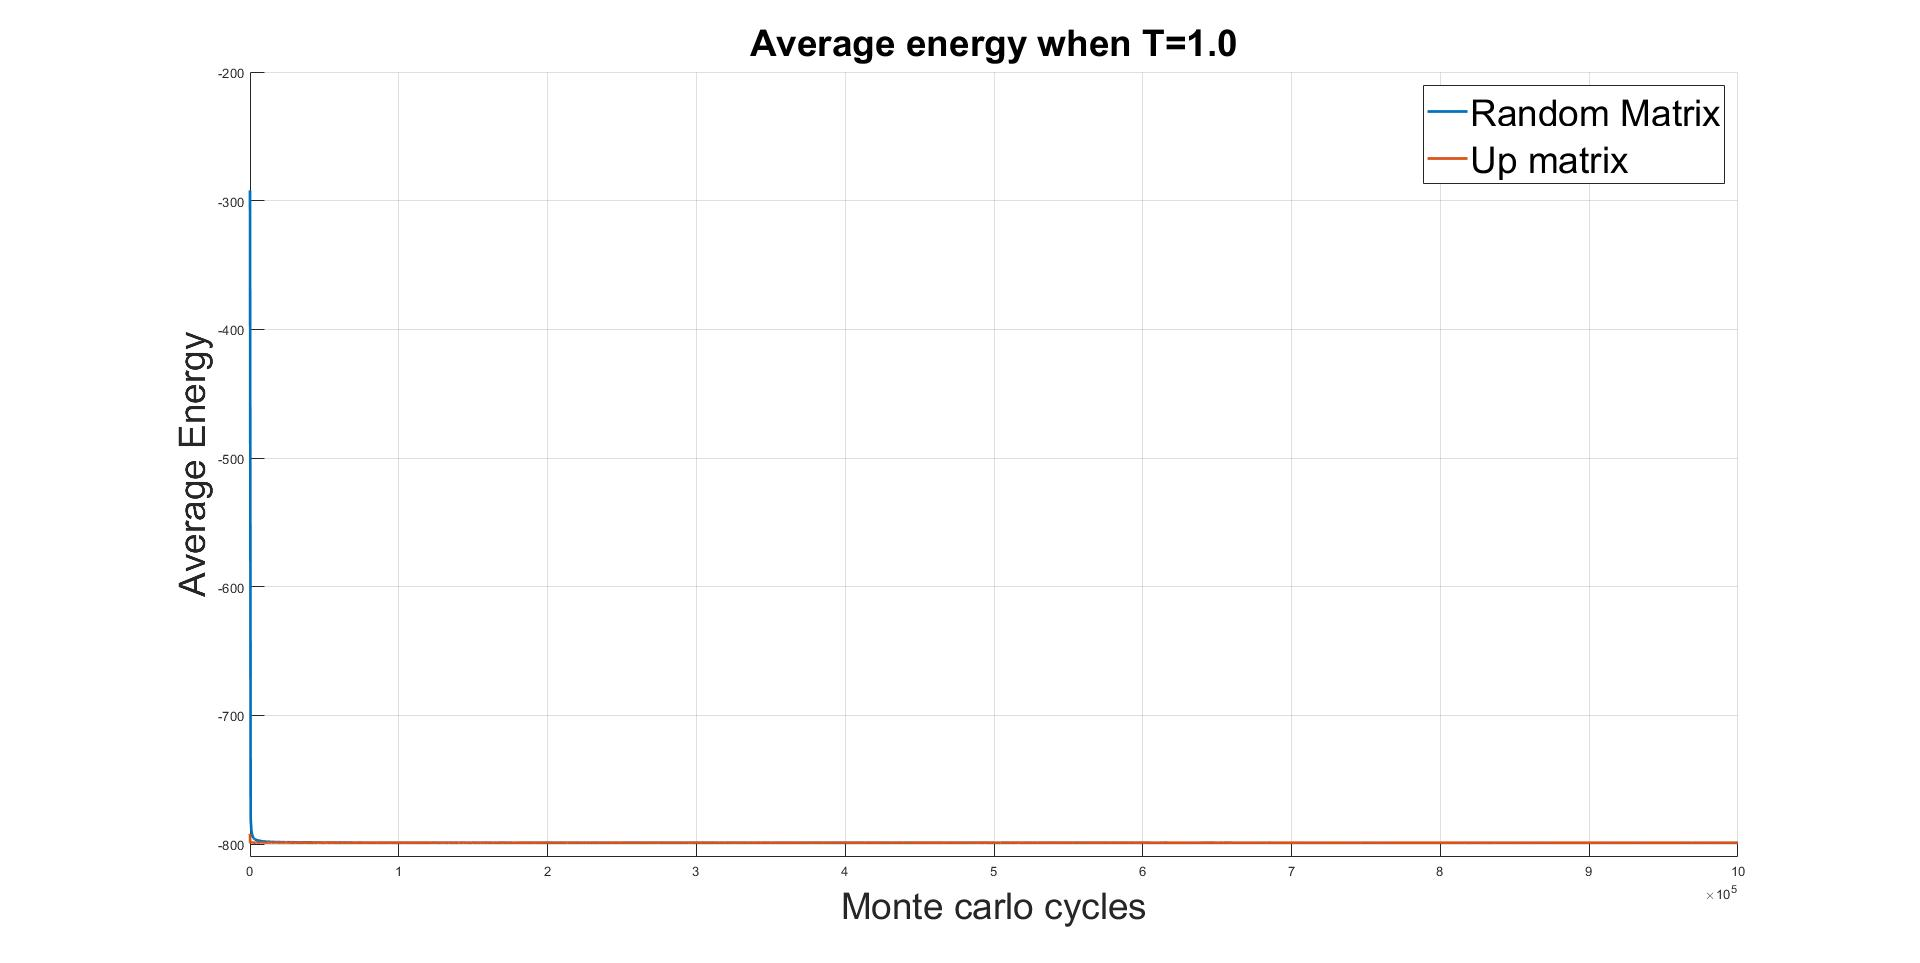
\includegraphics[scale=0.3]{avgEnergy1.jpg}
}
\caption{Development of average energy as a function of Monte Carlo cycles. Plotted at T=1.0 with an ordered and random matrix}
\label{fig:AverageEnergy1}
\end{figure}

\begin{figure} [H]
\centerline{
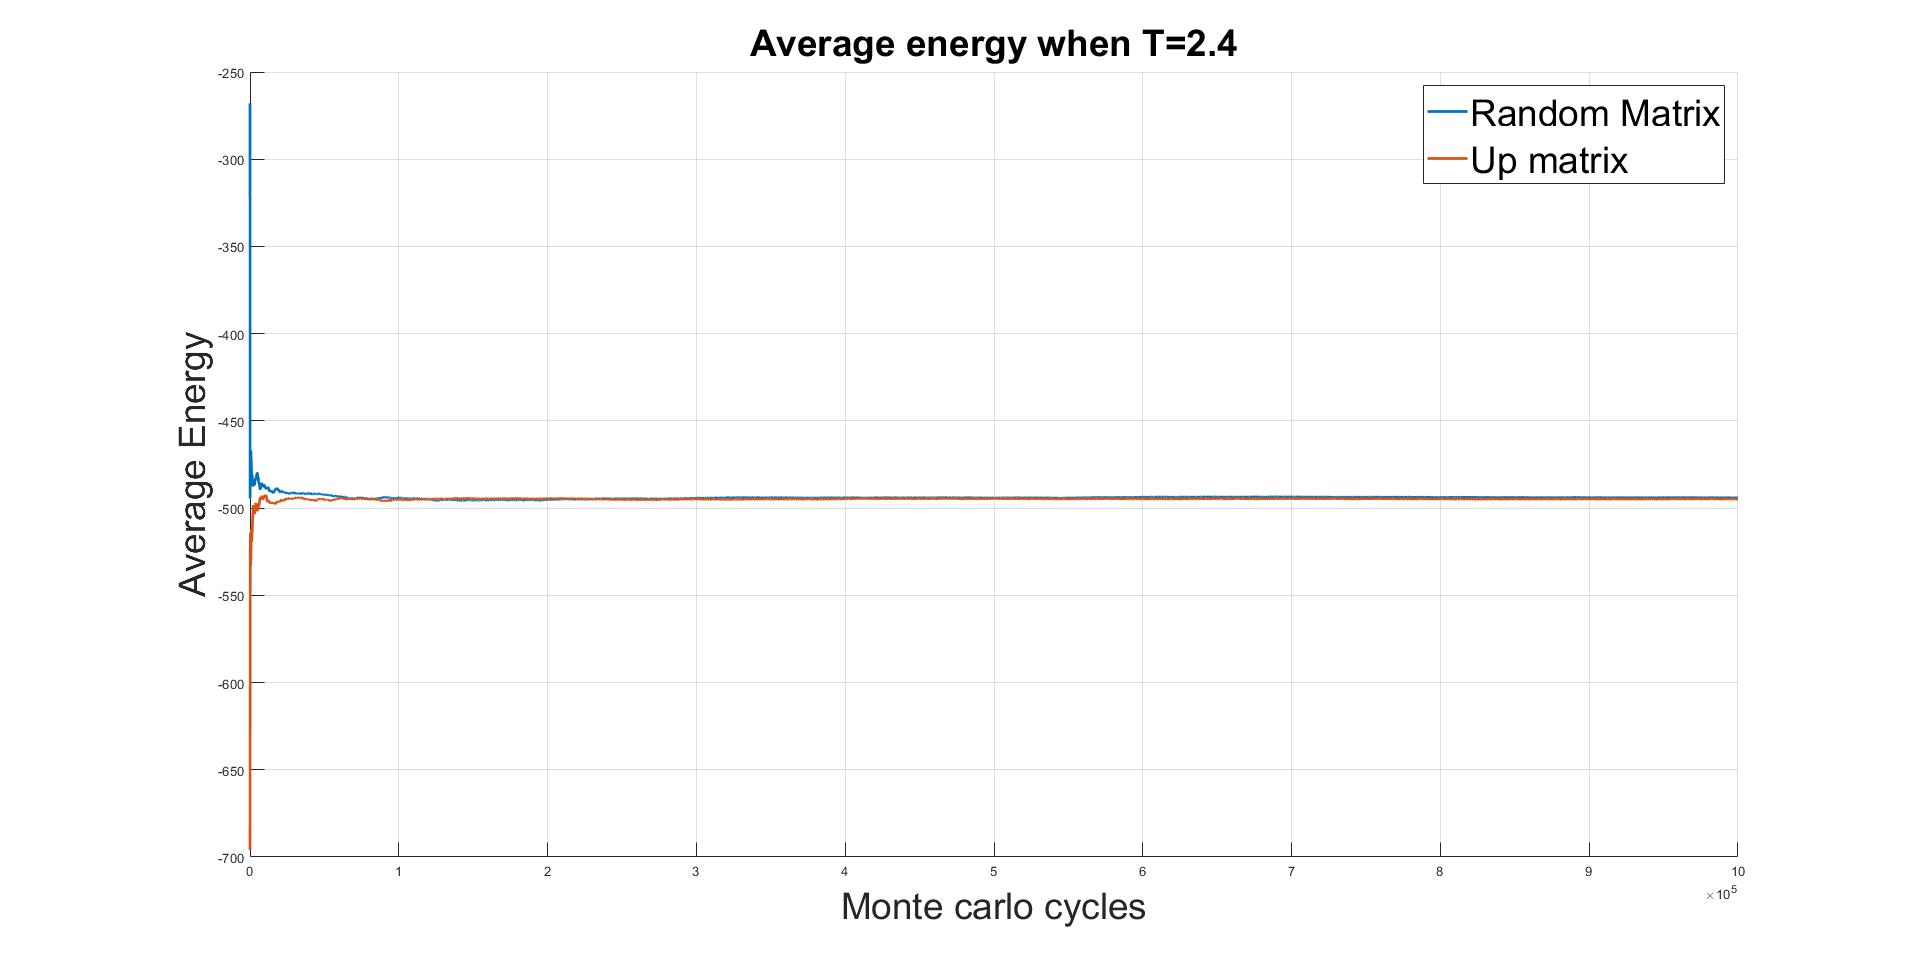
\includegraphics[scale=0.3]{avgEnergy24.jpg}
}
\caption{Development of average energy as a function of Monte Carlo cycles. Plotted at T=2.4 with an ordered and random matrix}
\label{fig:AverageEnergy24}
\end{figure}


\begin{figure} [H]
\centerline{
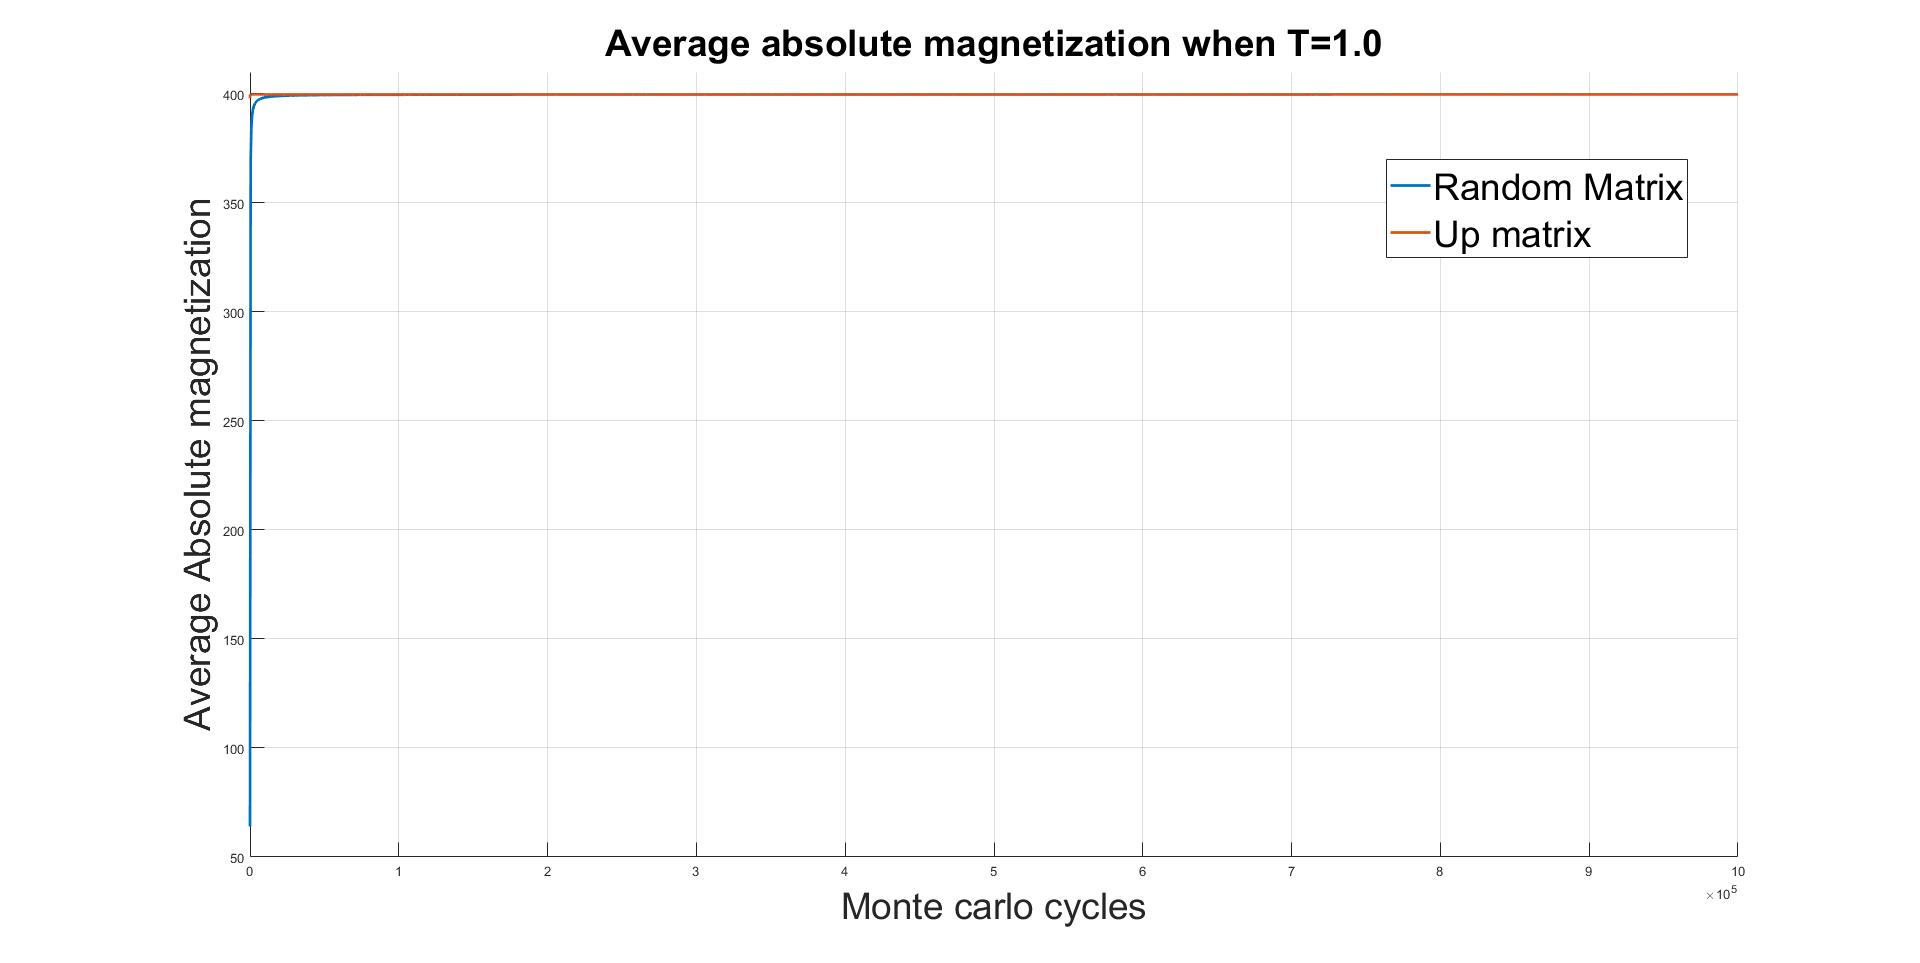
\includegraphics[scale=0.3]{avgMagn1.jpg}
}
\caption{Development of average absolute magnetization as a function of Monte Carlo cycles. Plotted at T=1.0 with an ordered and random matrix}
\label{fig:AverageMagn1}
\end{figure}


\begin{figure} [H]
\centerline{
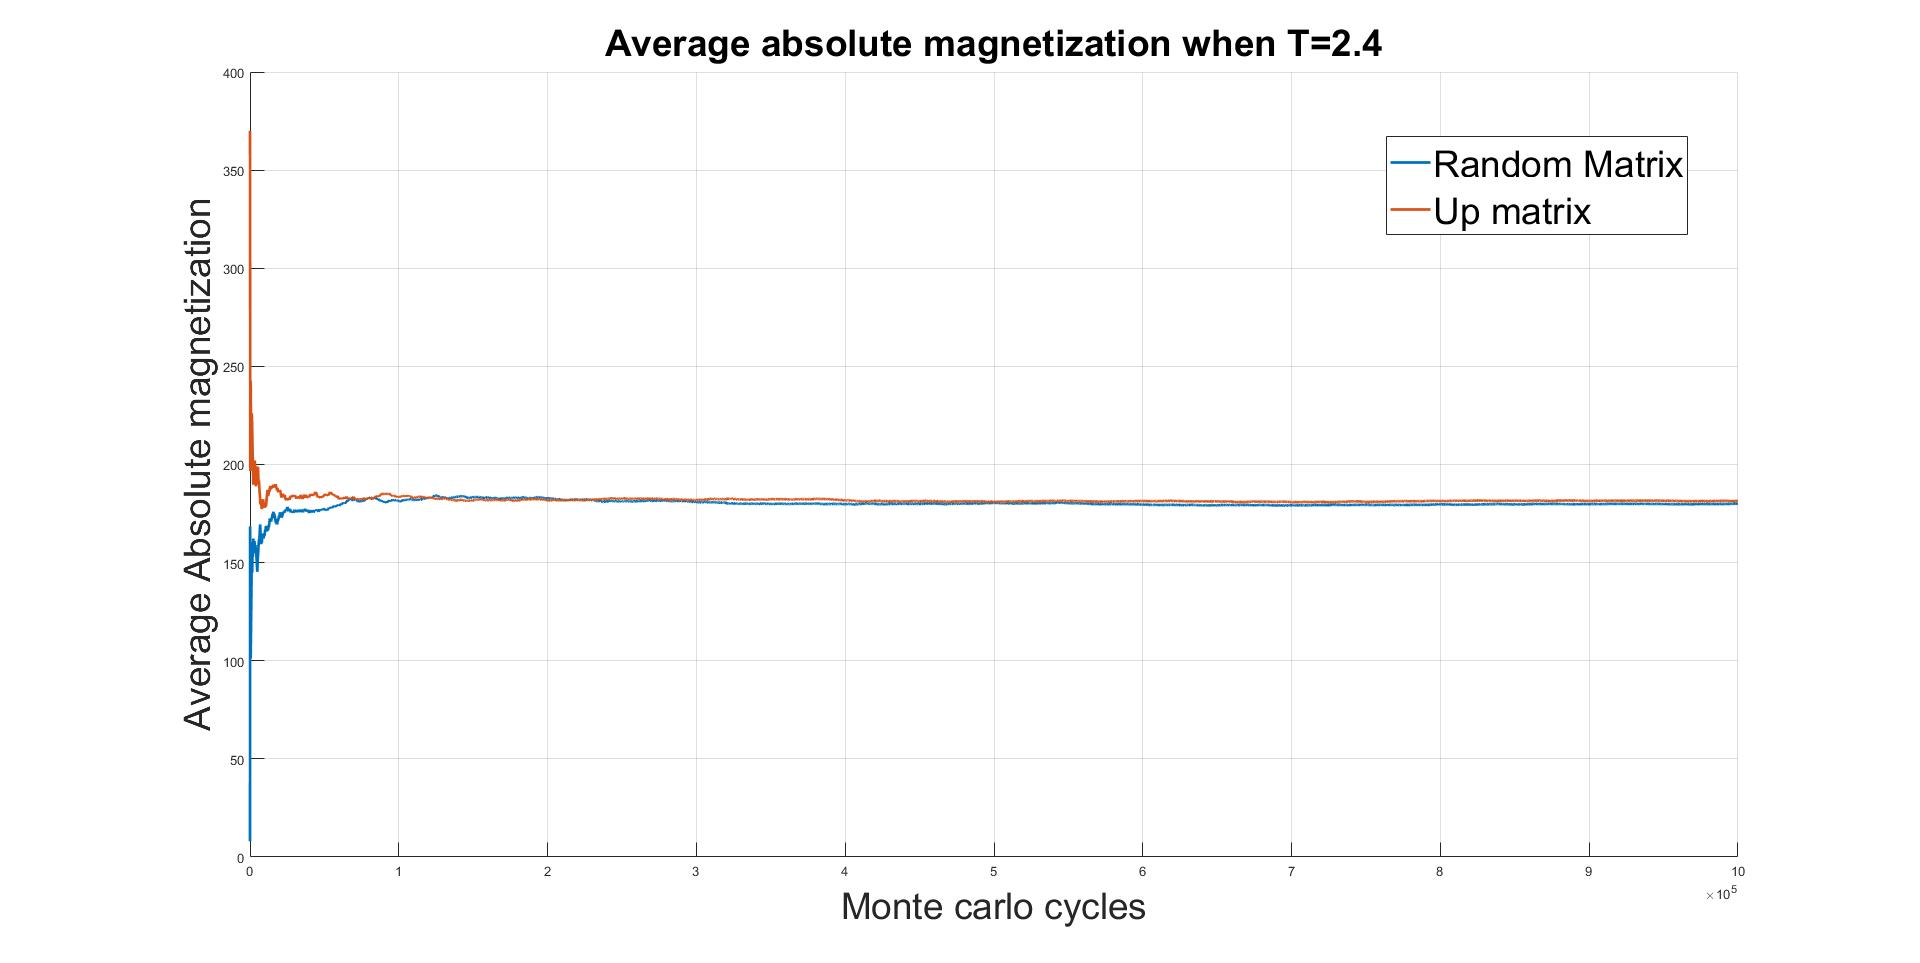
\includegraphics[scale=0.3]{avgMagn24.jpg}
}
\caption{Development of average absolute magnetization as a function of Monte Carlo cycles. Plotted at T=2.4 with an ordered and random matrix}
\end{figure}



\noindent All figures of energy and magnetization were plotted with 1 000 000 Monte Carlo cycles and written to file for every 2500 points 


\begin{figure} [H]
\centerline{
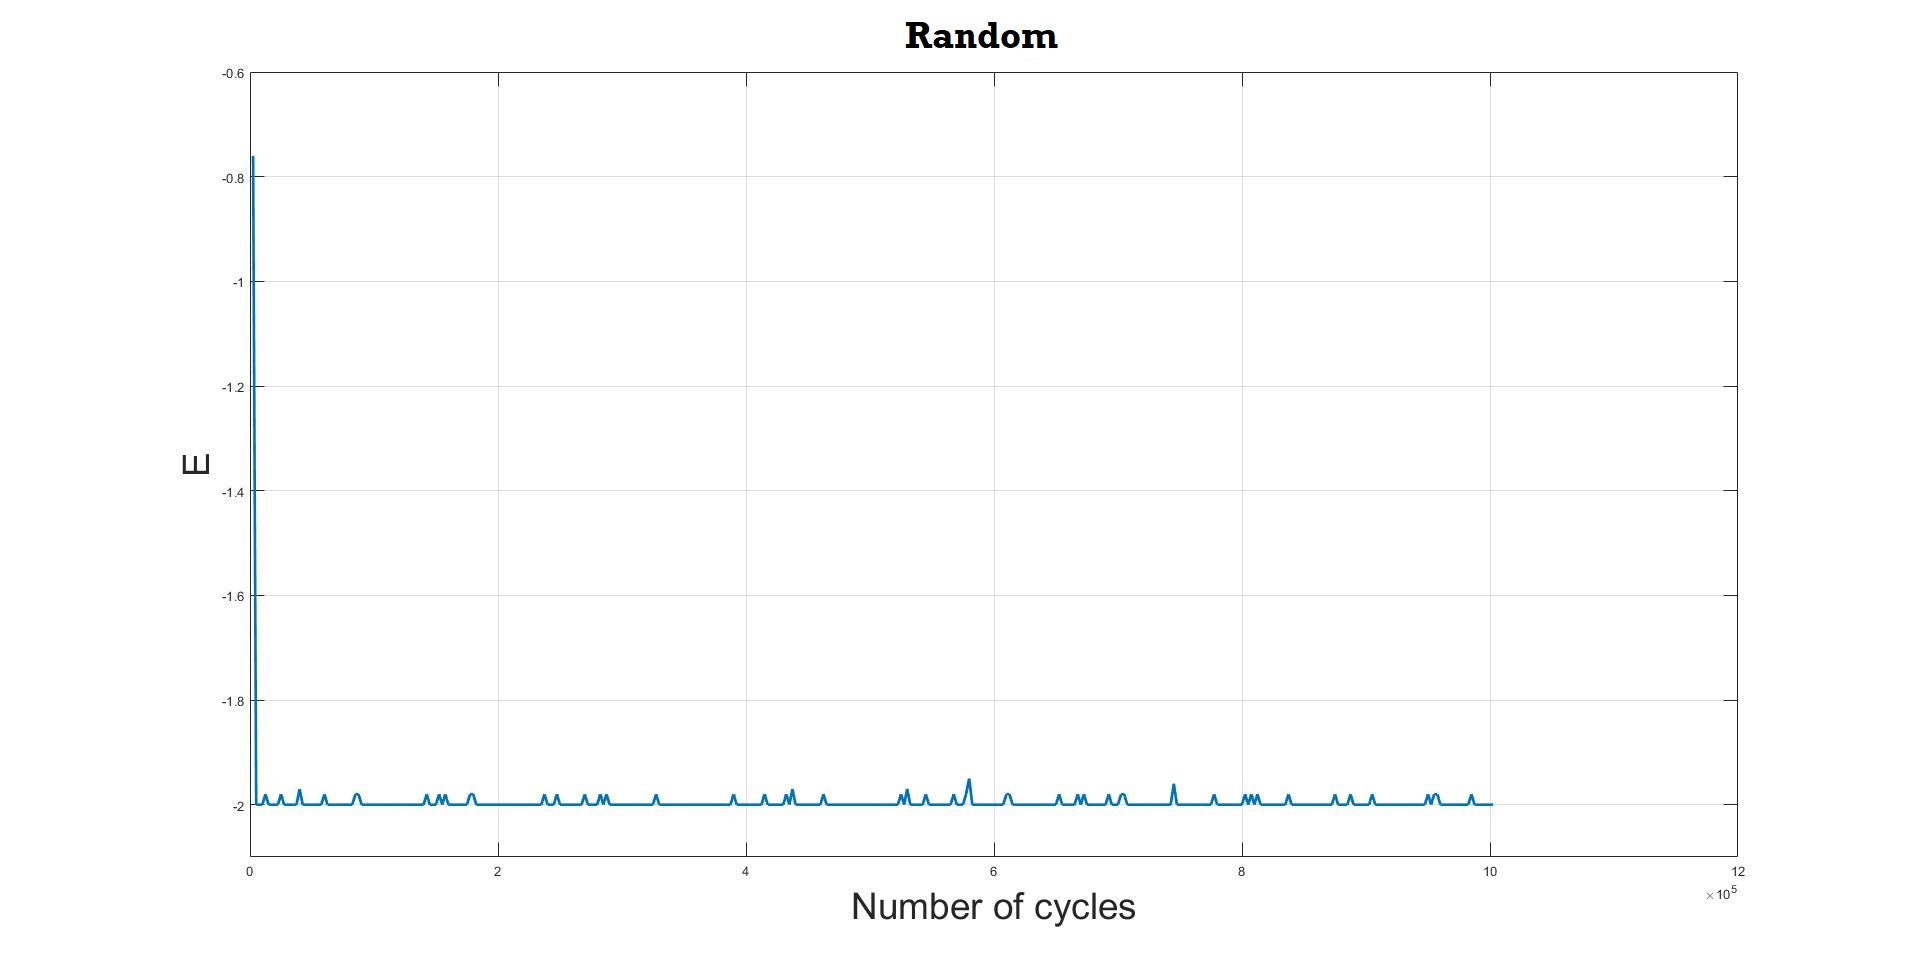
\includegraphics[scale=0.15]{RANDOMenergy1.jpg}
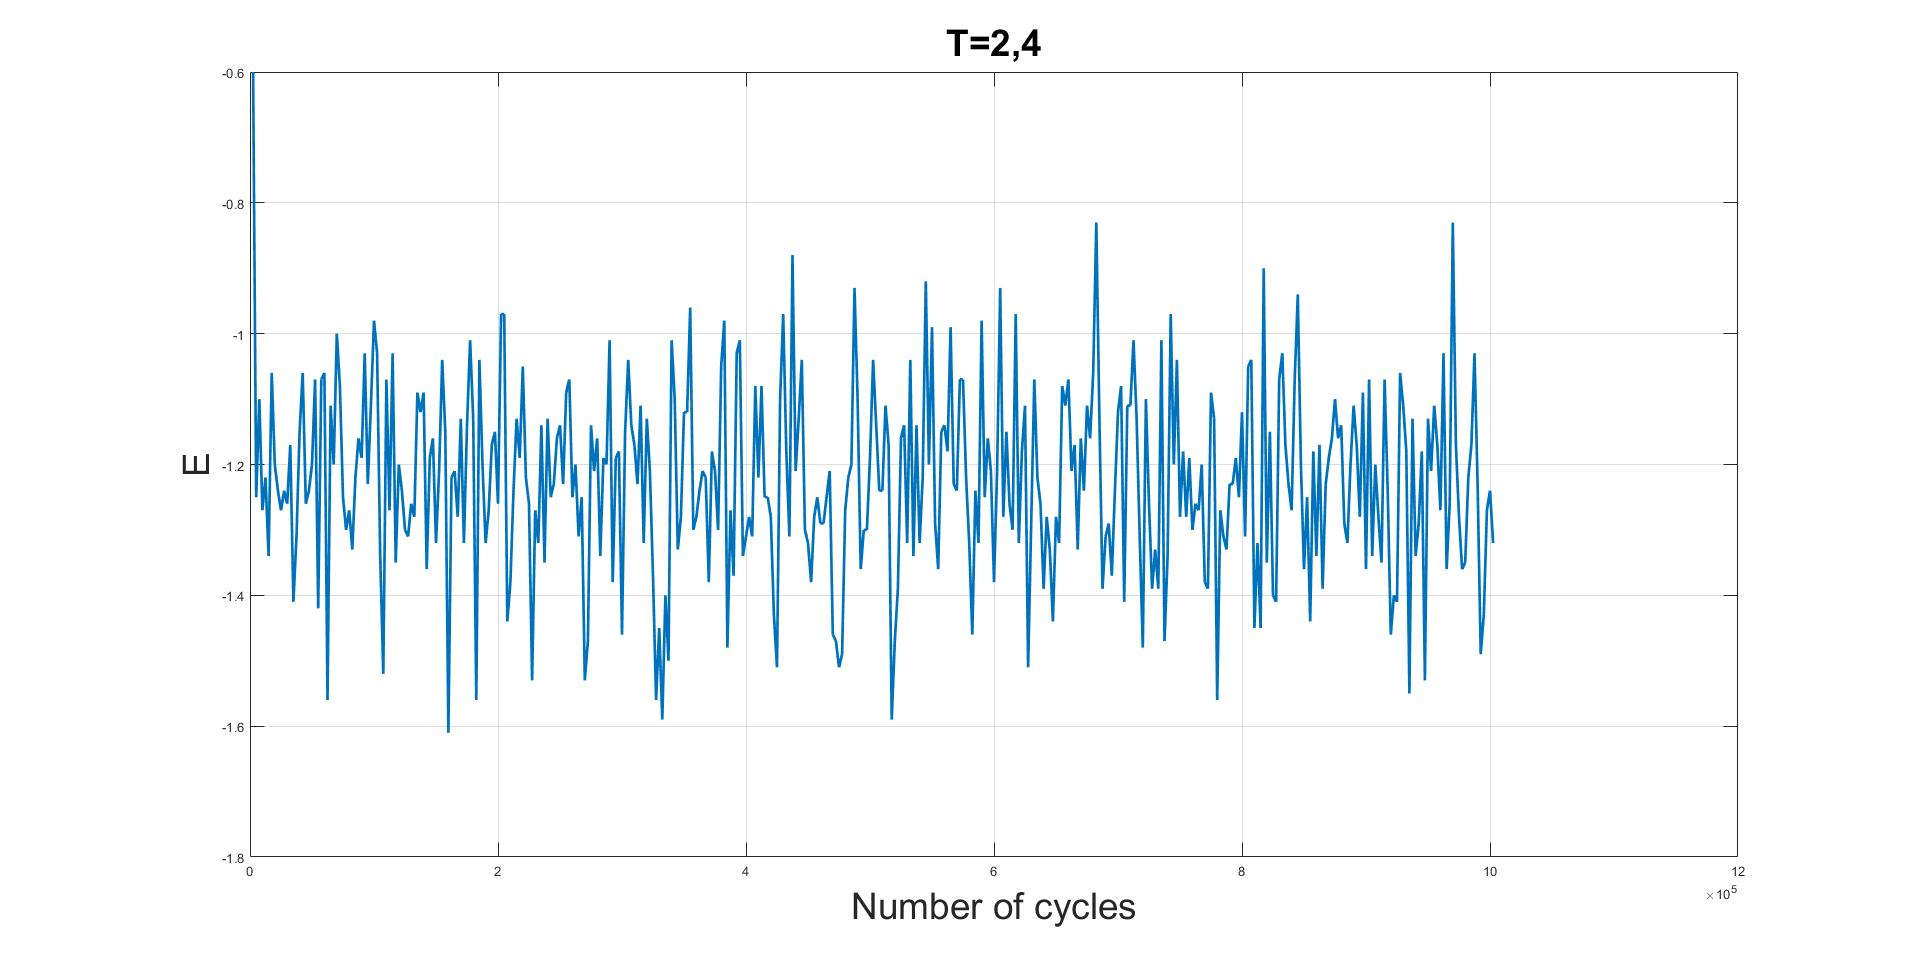
\includegraphics[scale=0.15]{RANDOMenergy24.jpg}
}
\caption{Energy of random initial matrix per lattice point plotted against number of monte carlo cycles for T=1.0 and T=2.4}
\label{fig:RandomEnergy}
\end{figure}


\begin{figure} [H]
\centerline{
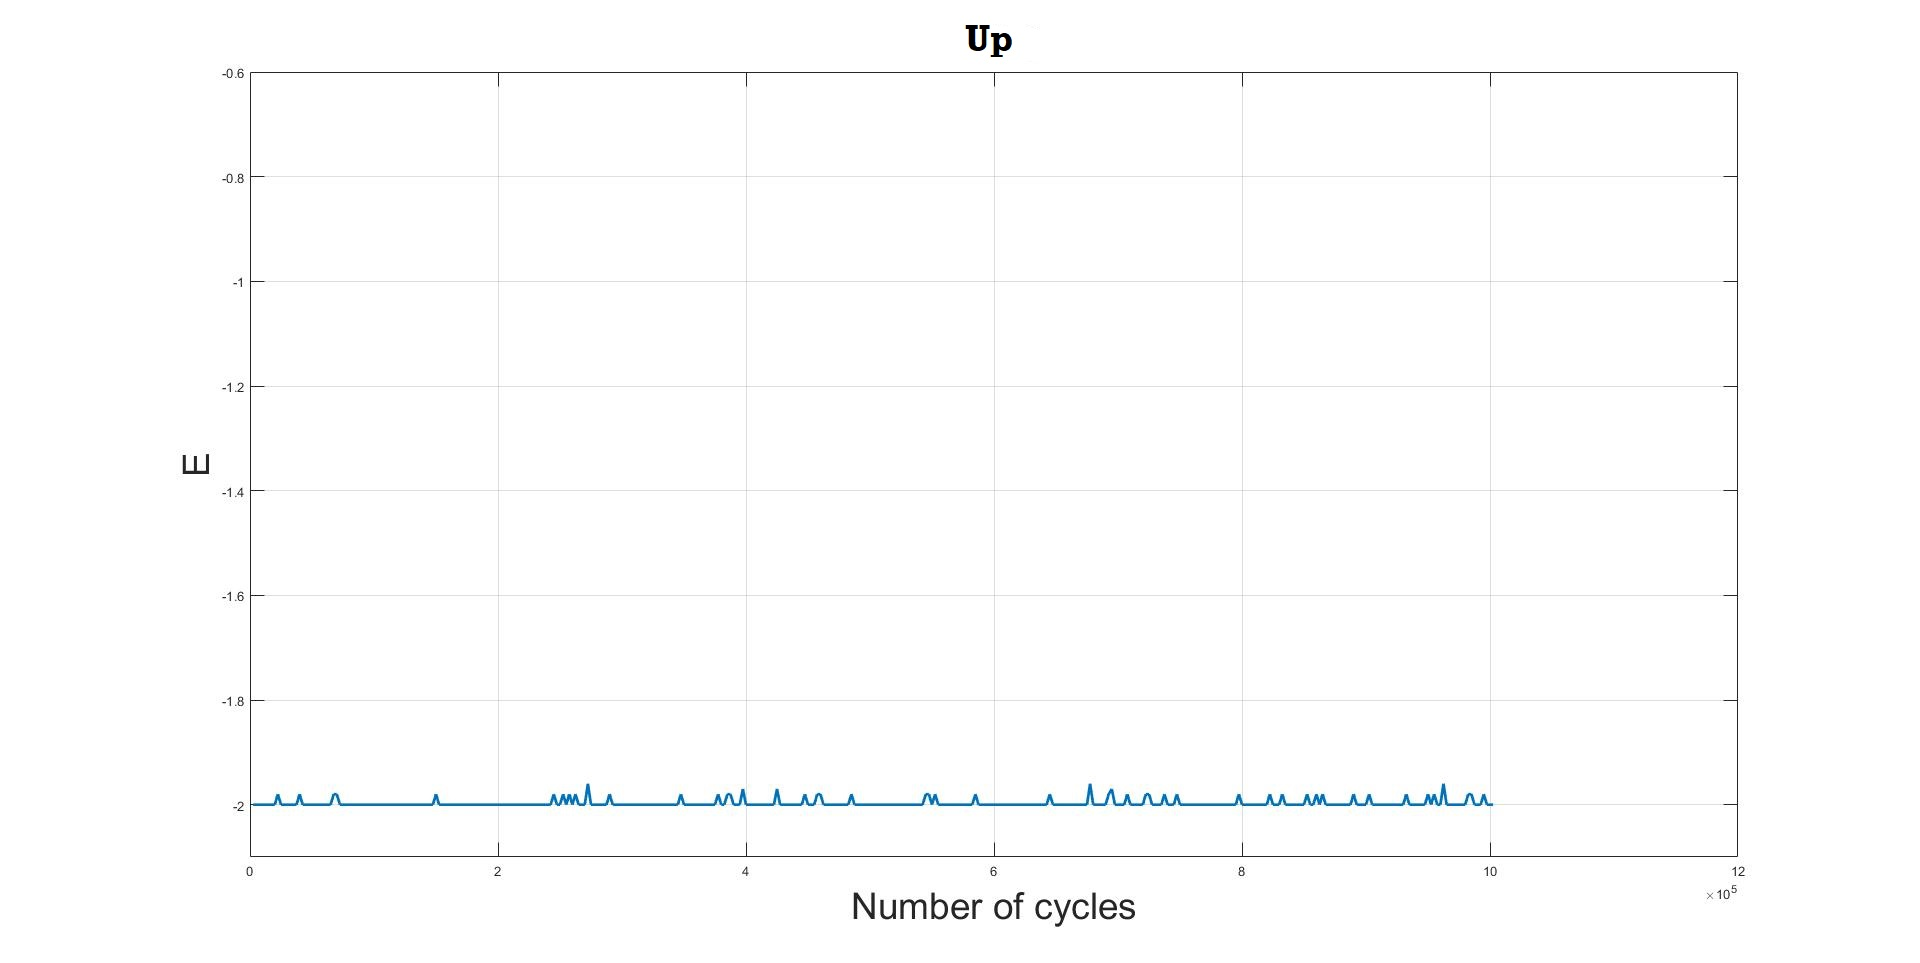
\includegraphics[scale=0.15]{UPenergy1.jpg}
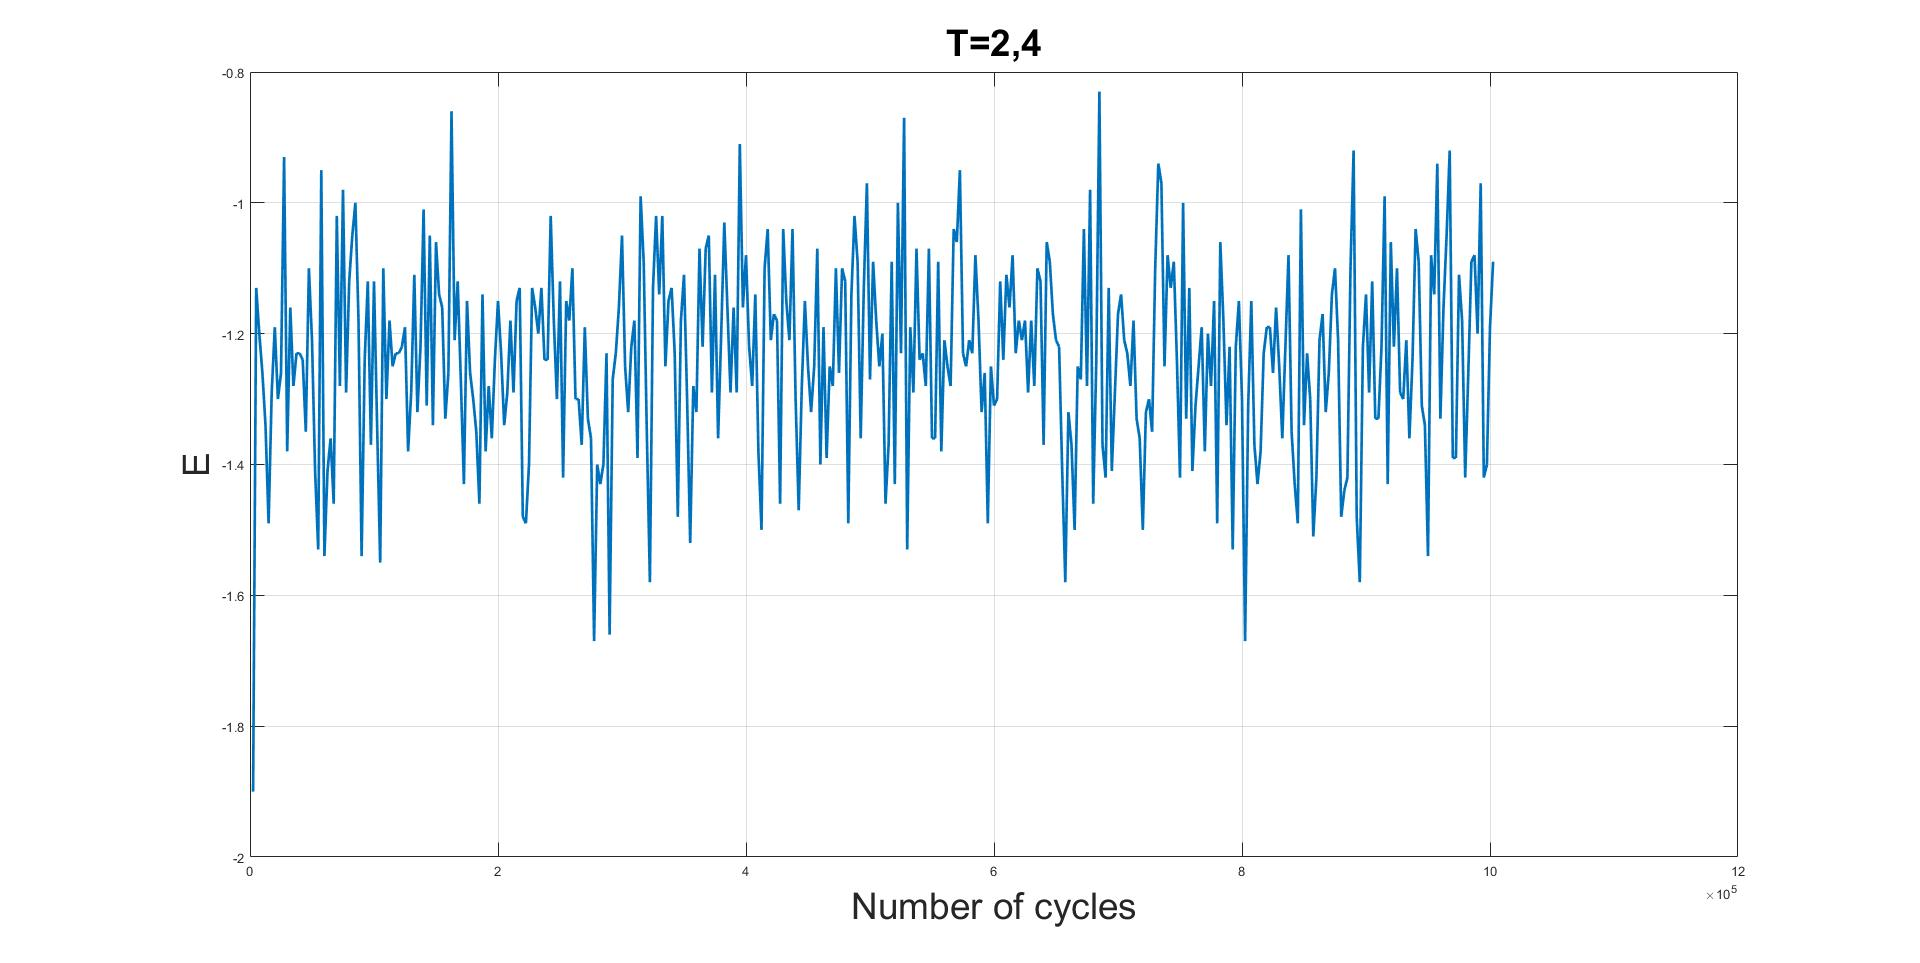
\includegraphics[scale=0.15]{UPenergy24.jpg}
}
\caption{Energy of all spins up initital matrix plotted against number of monte carlo cycles}
\label{fig:UpEnergy}
\end{figure}

\noindent It is clear to see in \figref{RandomEnergy} and \figref{UpEnergy} that the energy quickly converges to a steady state around $-2$ when $T=1.0$. For the all up initial configuration, it is already at this steady state. This equilibrium state is confined to a small number of energy levels. For $T=2.4$ the energy also converges to an equilibrium state, but the energy fluctuates more than for lower temperature. This is to be expected, because there is more energy in the system, and will be elaborated further later in the report. 

\begin{figure} [H]
\centerline{
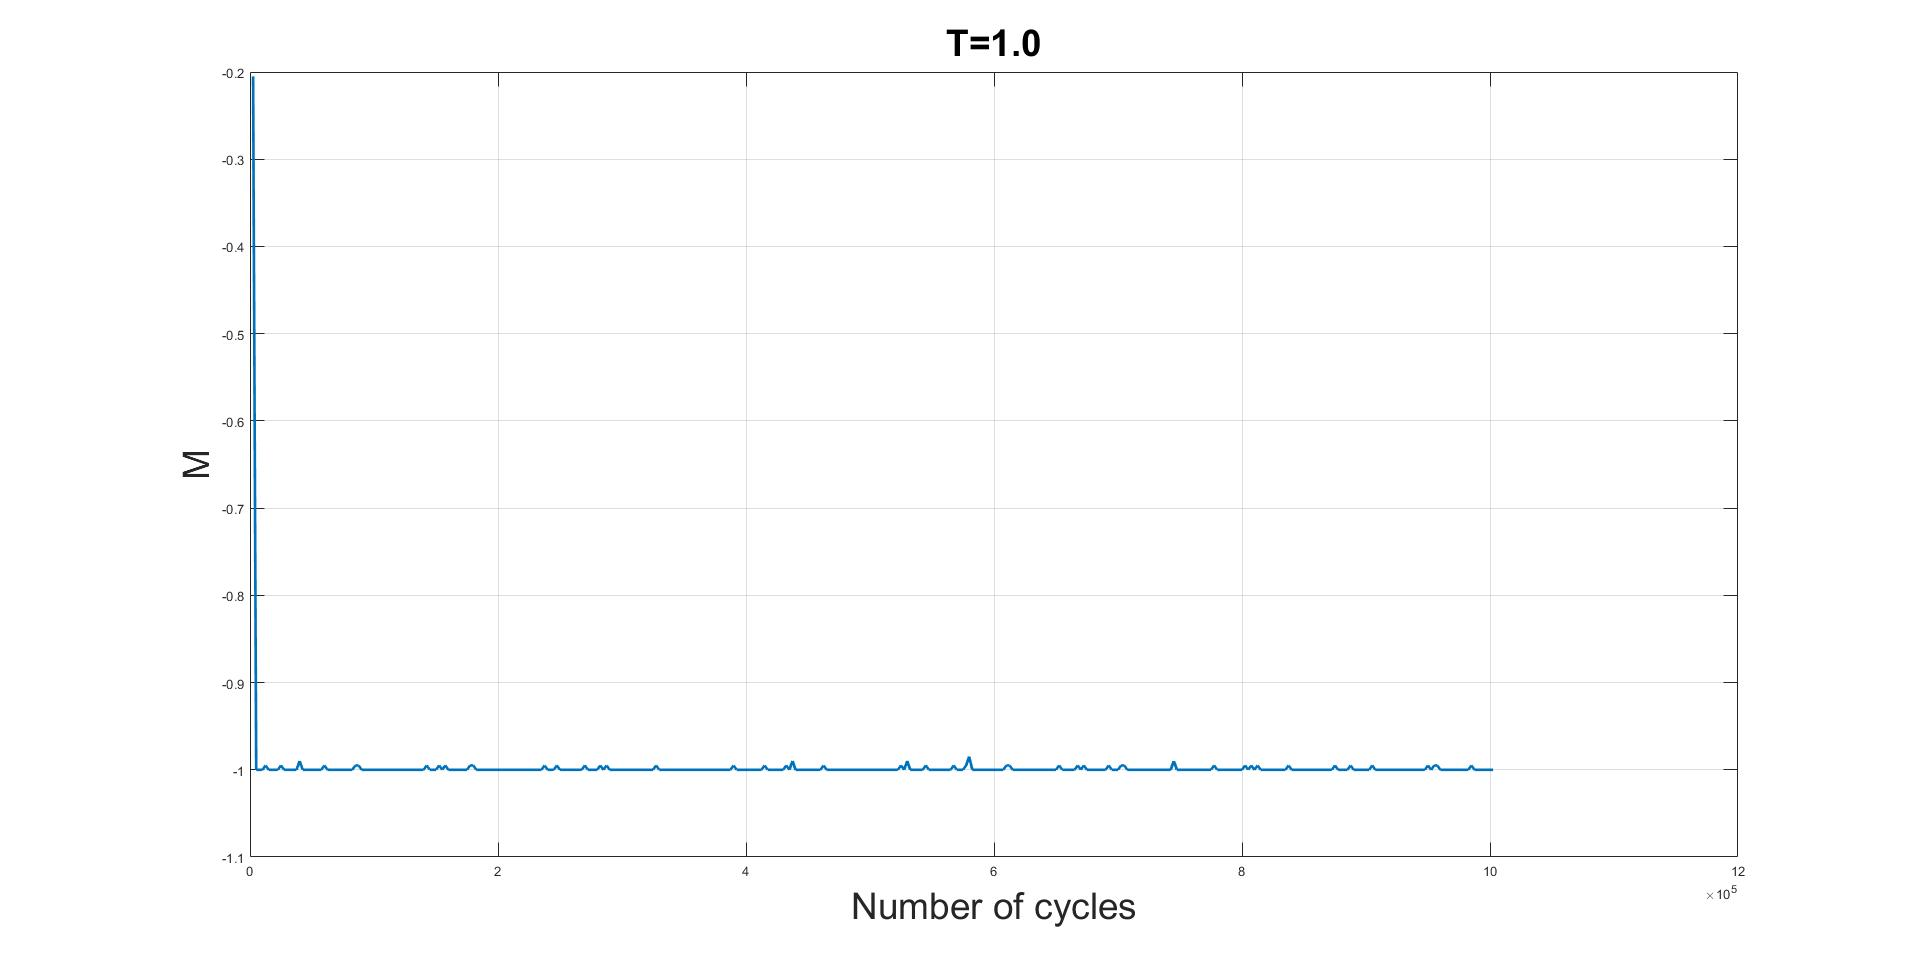
\includegraphics[scale=0.15]{RANDOMmag1notabs.jpg}
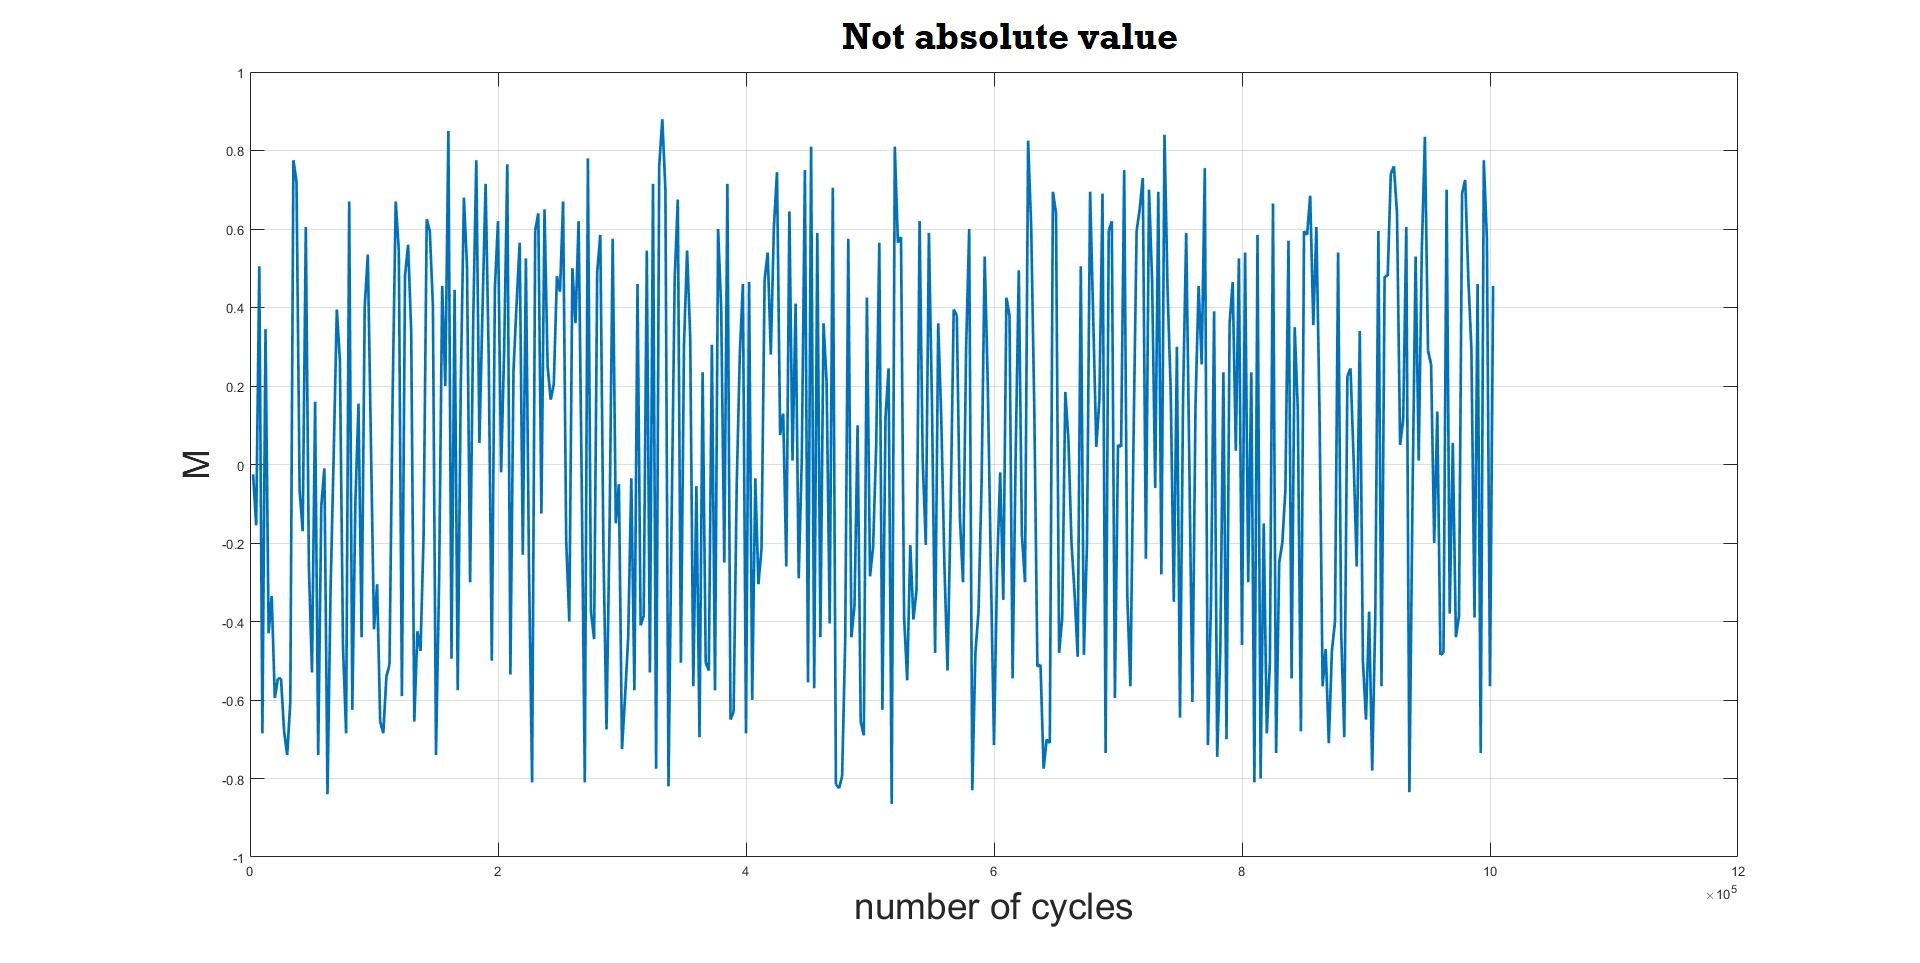
\includegraphics[scale=0.15]{RANDOMmag24notabs.jpg}
}
\caption{Development of magnetization with random starting matrices for increasing monte carlo cycles.}
\label{fig:RandomMagNotAbs}
\end{figure}


\begin{figure} [H]
\centerline{
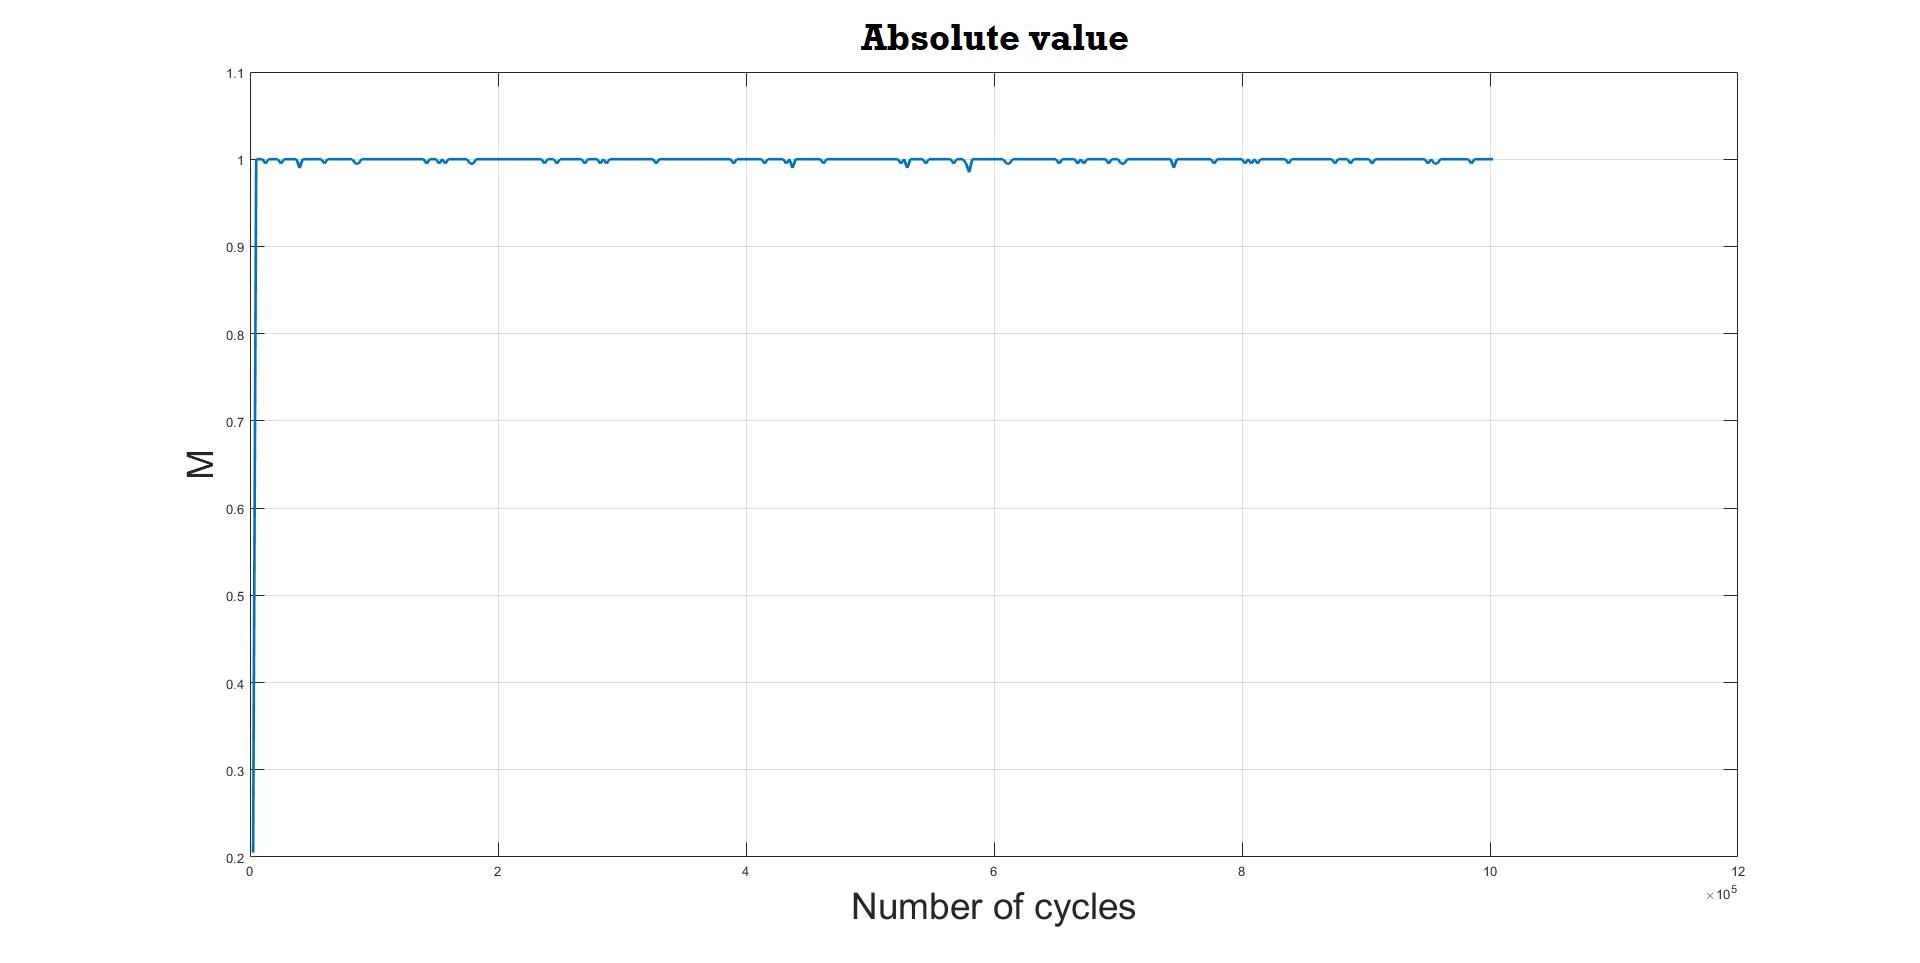
\includegraphics[scale=0.15]{RANDOMmag1abs.jpg}
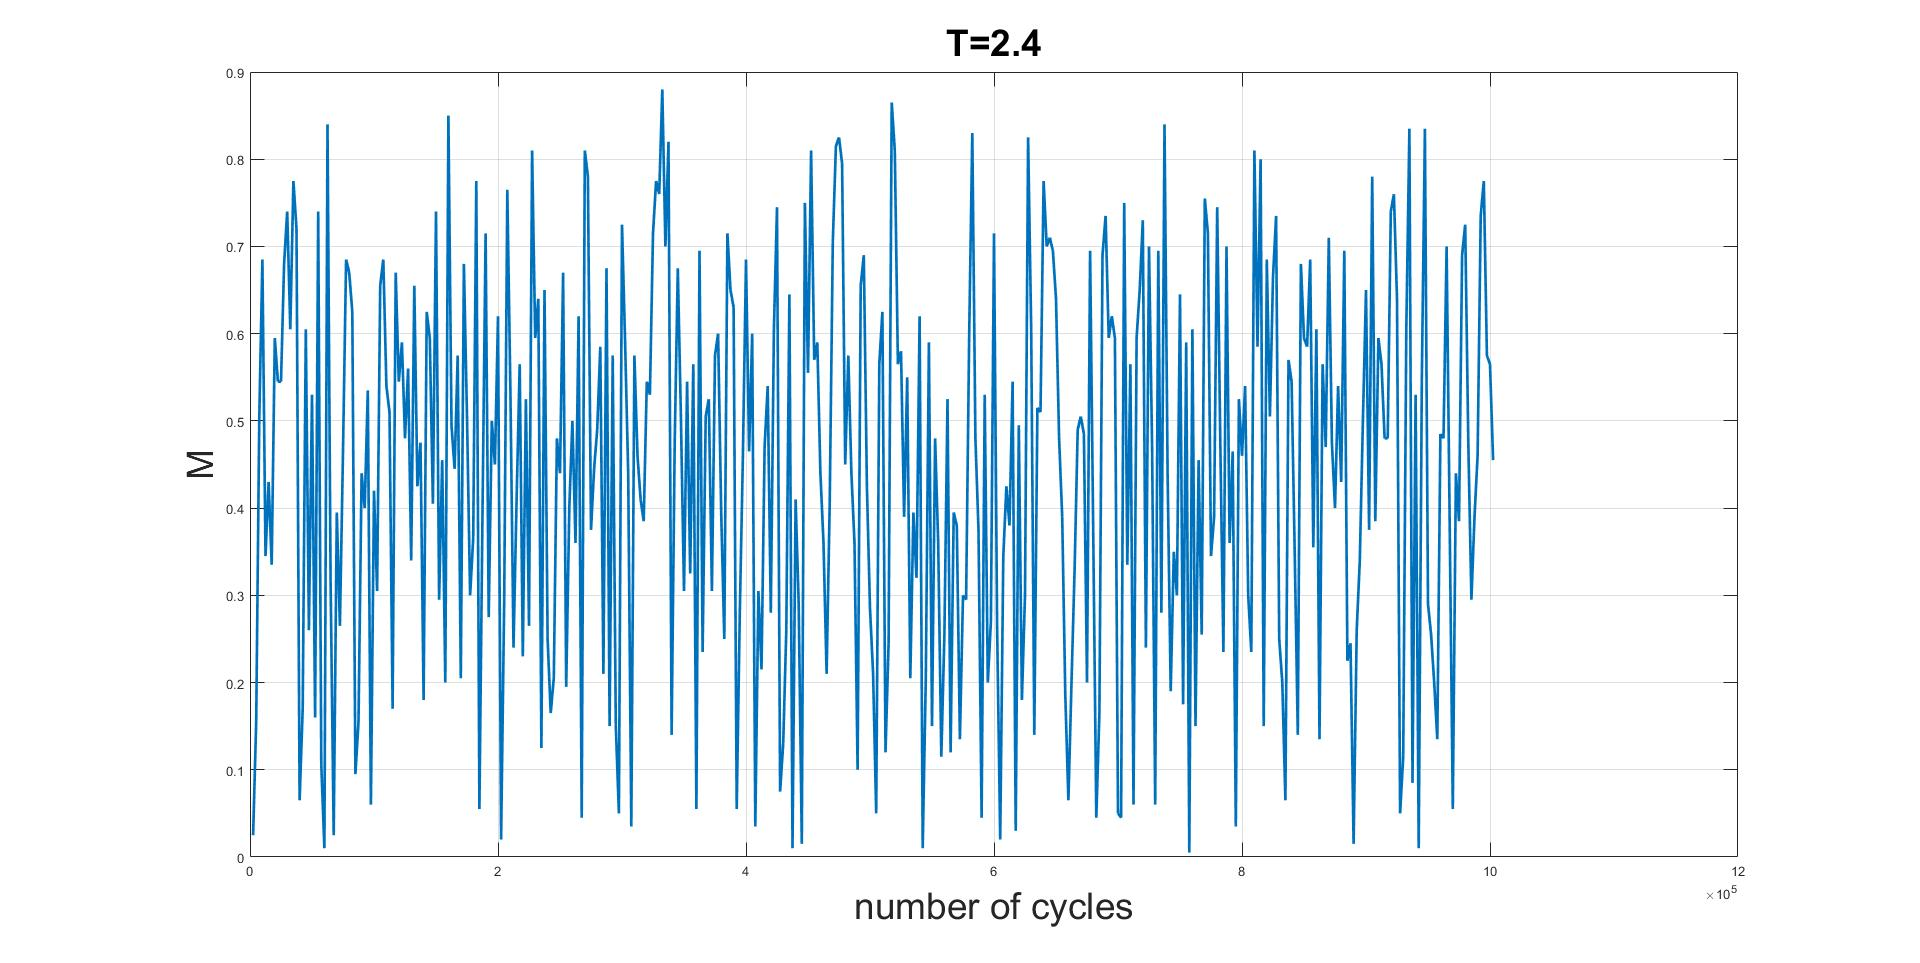
\includegraphics[scale=0.15]{RANDOMmag24abs.jpg}
}
\caption{Development of absolute magnetization with random starting matrices for increasing Monte Carlo cycles.}
\label{fig:RandomMagAbs}
\end{figure}


\begin{figure} [H]
\centerline{
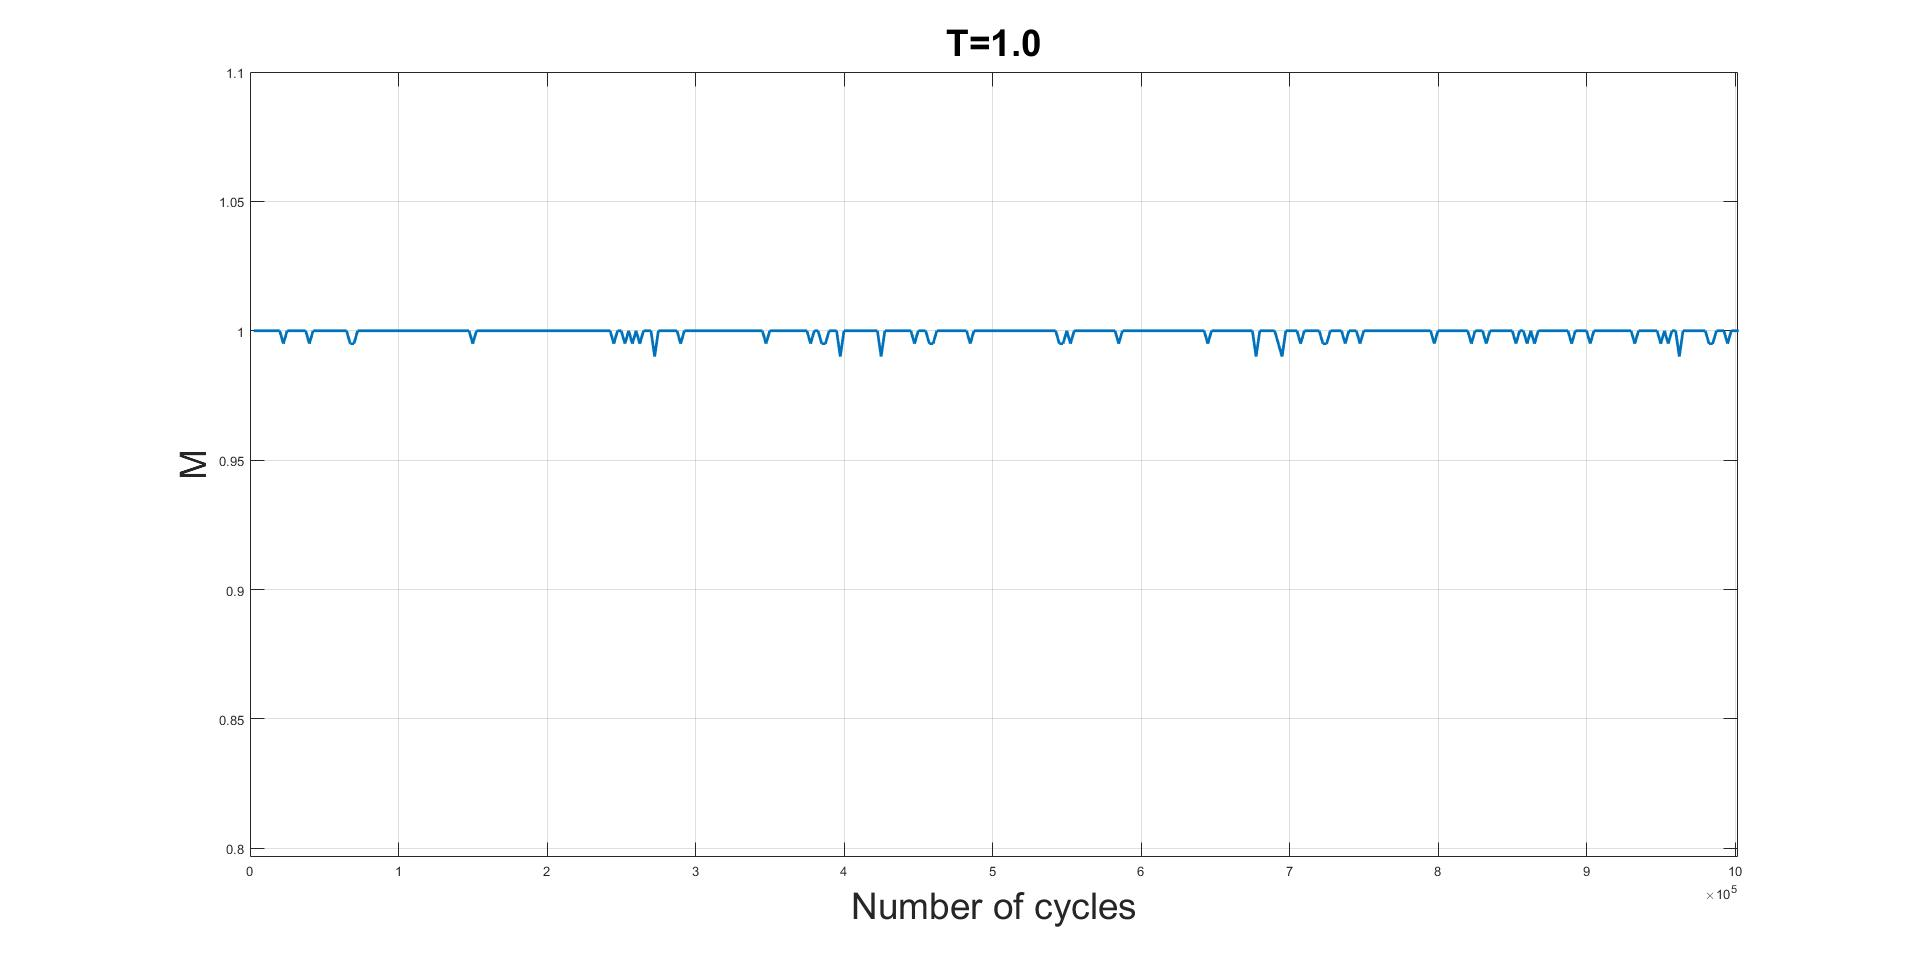
\includegraphics[scale=0.15]{UPmag1notabs.jpg}
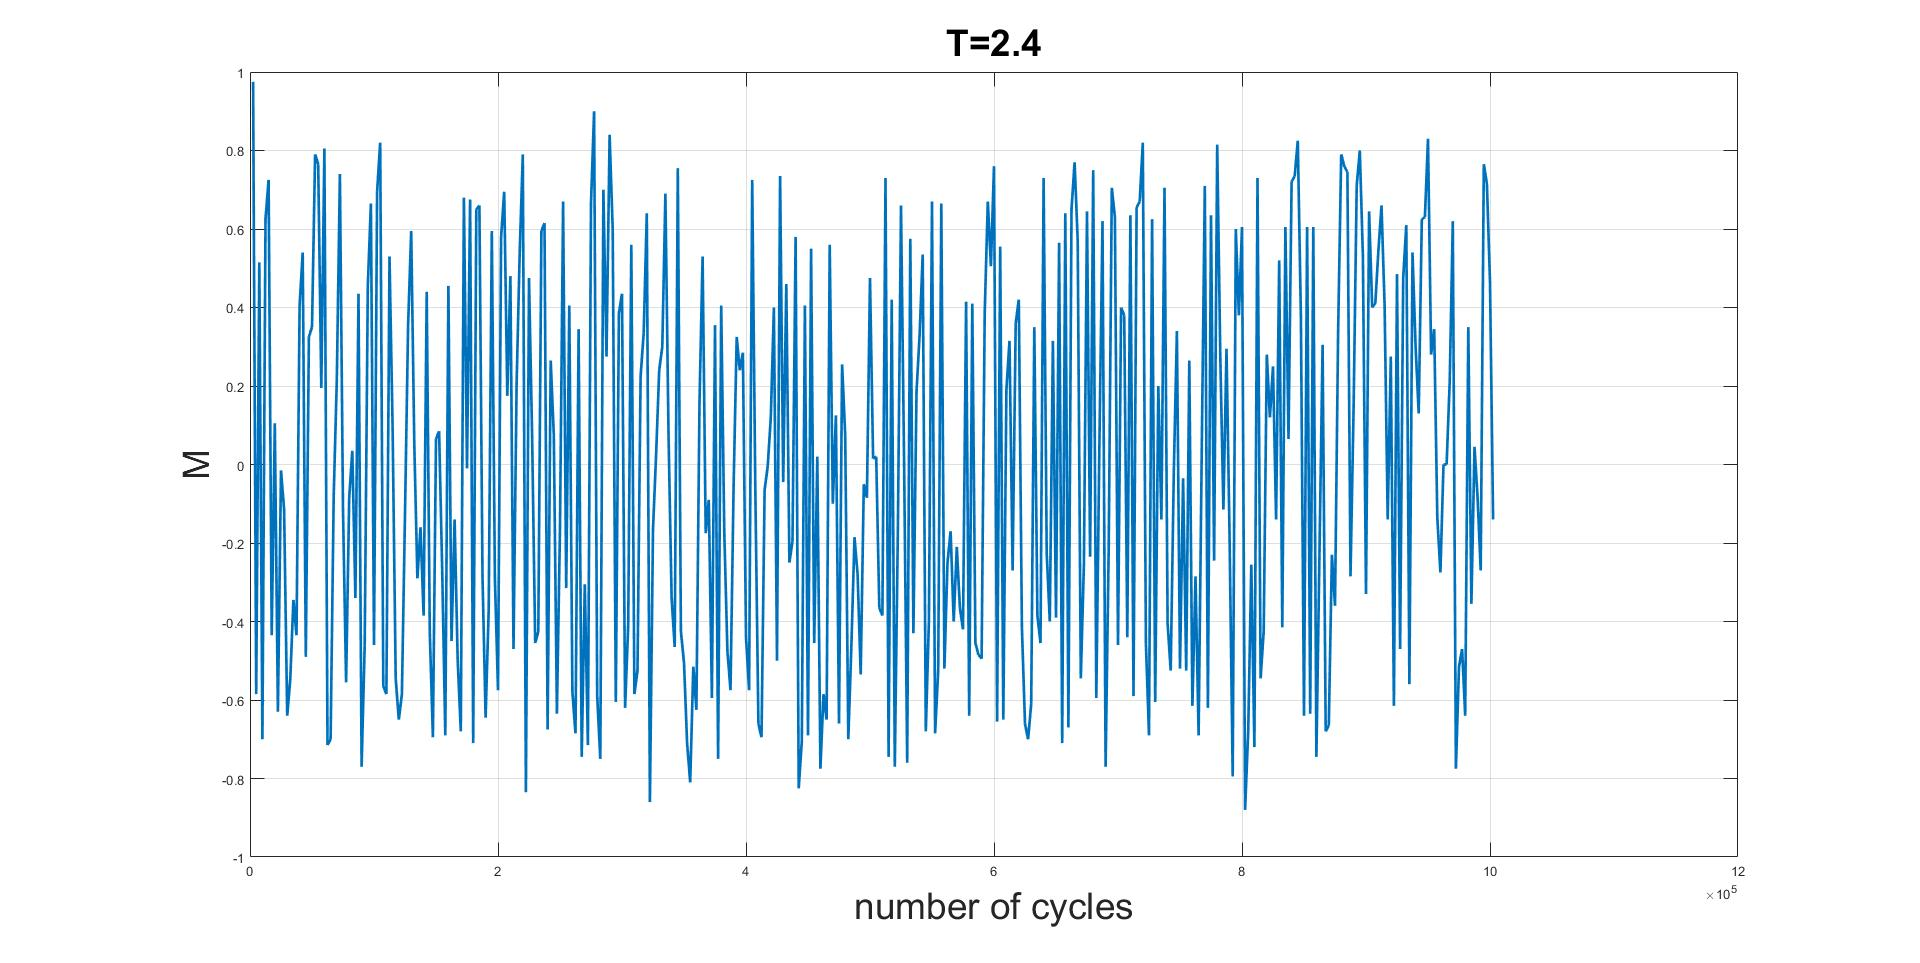
\includegraphics[scale=0.15]{UPmag24notabs.jpg}
}
\caption{Development of magnetization with all up starting matrices for increasing Monte Carlo cycles}
\label{fig:UpMagNotAbs}
\end{figure}


\begin{figure} [H]
\centerline{
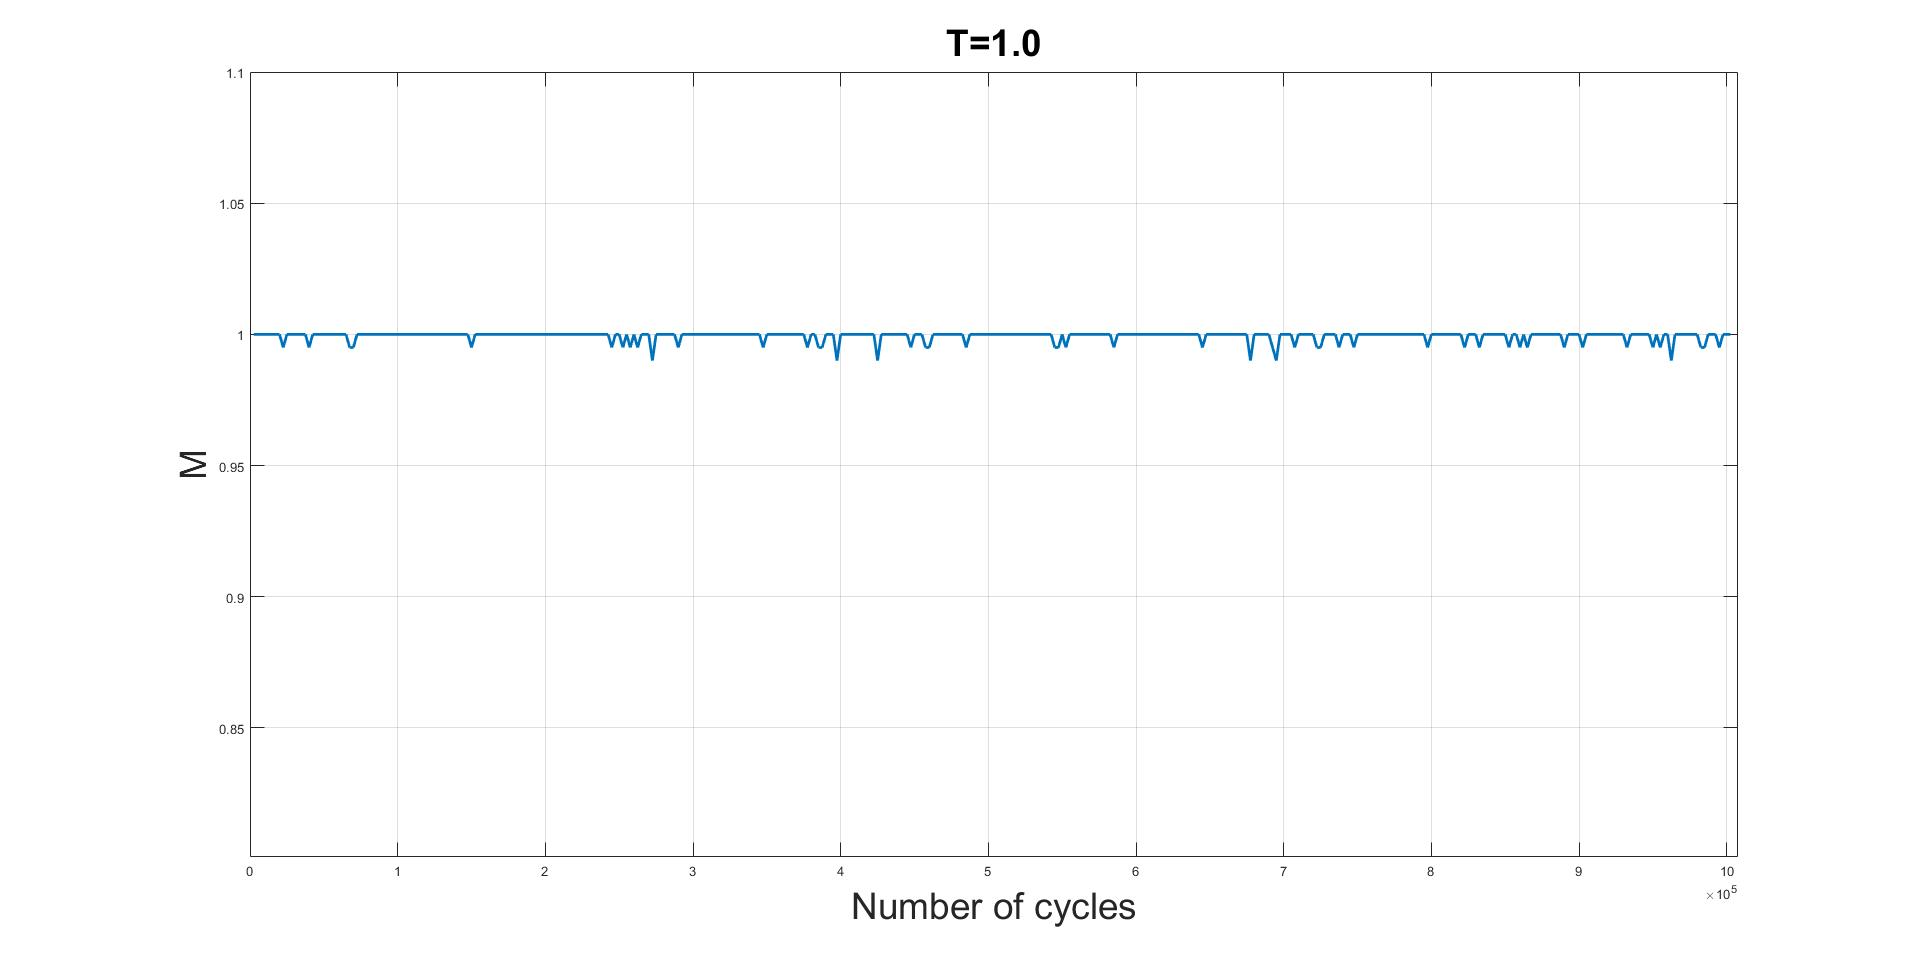
\includegraphics[scale=0.15]{UPmag1abs.jpg}
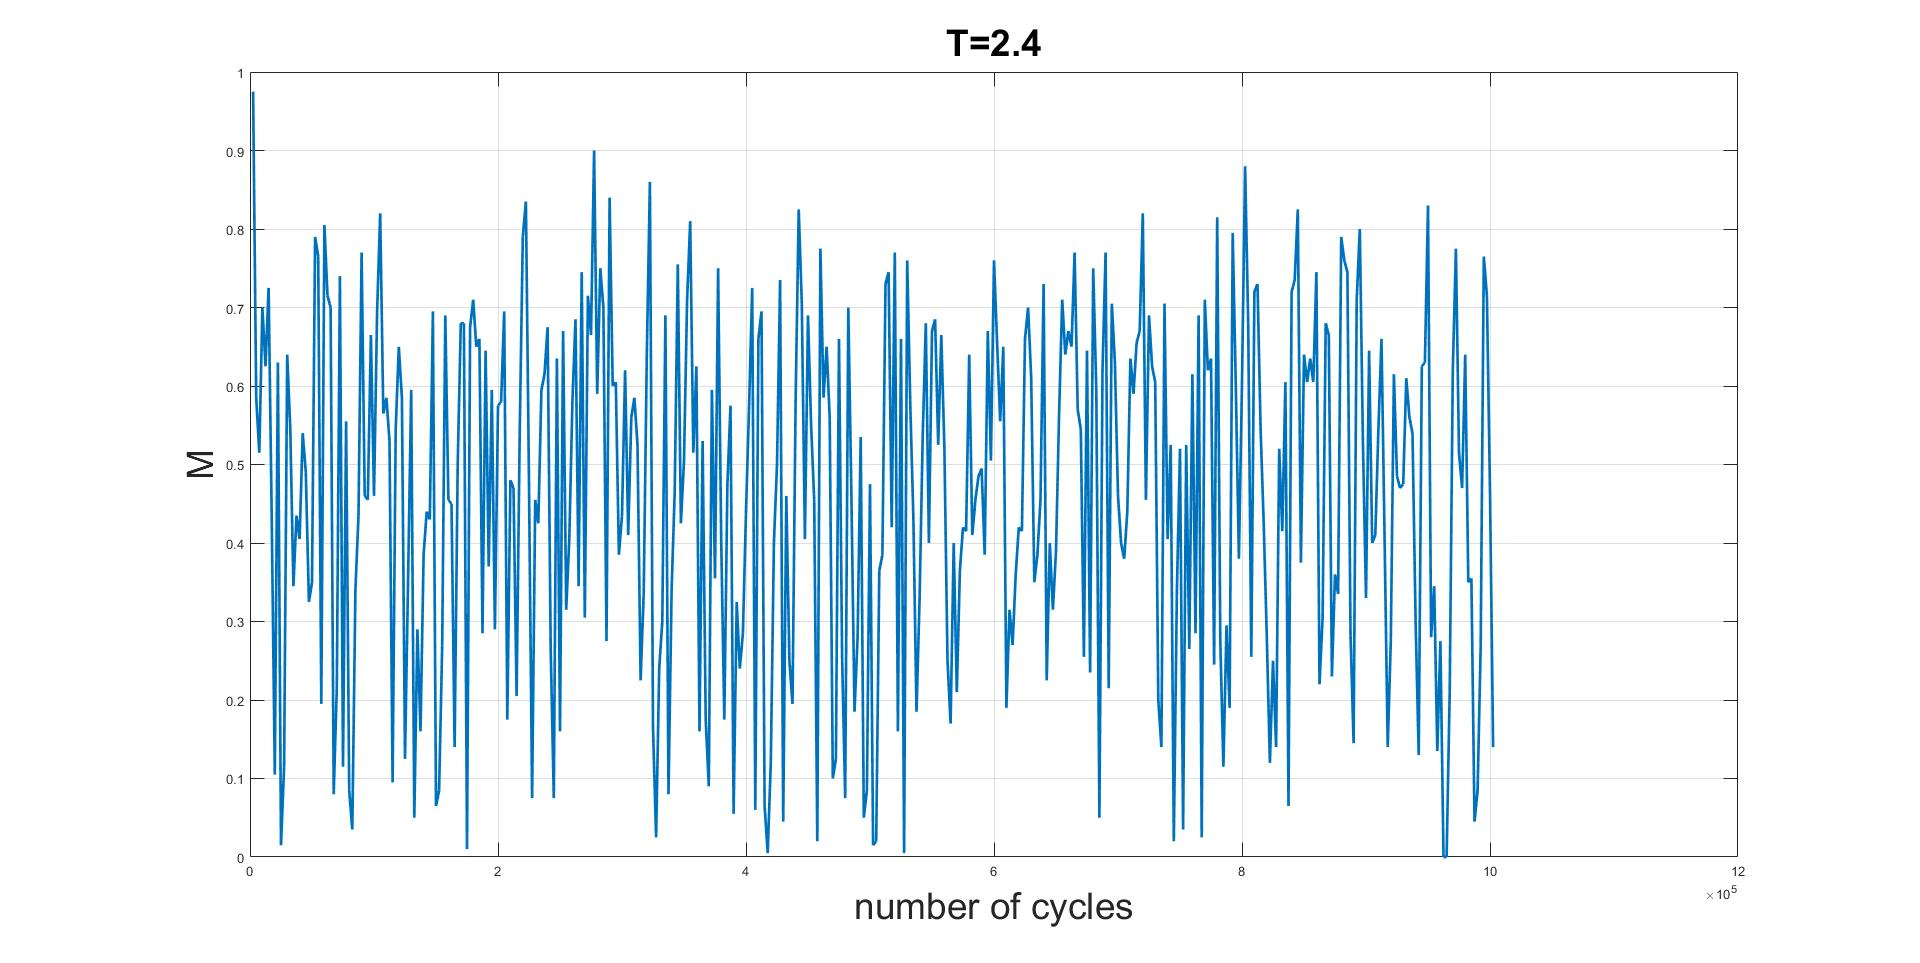
\includegraphics[scale=0.15]{UPmag24abs.jpg}
}
\caption{Development of absolute magnetization with all up starting matrices for increasing Monte Carlo cycles.}
\label{fig:UpMagnetizm}
\end{figure}
\noindent \figref{RandomMagNotAbs}, \figref{RandomMagAbs}, \figref{UpMagNotAbs} and \figref{UpMagnetizm} shows that the magnetization behaves similarly for $T=1.0$ in all the cases. There is no difference at all when taking the absolute value for the all up initial matrix, because the magnetism is continuously positive to begin with. When the starting matrix is random, the first Monte Carlo cycles is used to reach the equilibrium state. As the random matrix in this instance is closer to an equilibrium state where all the spins point down, it will tend towards this state instead of the configuration with all spins up. These two states have the same energy, hence both states serve as a valid energy equilibrium. \\

\noindent When $T=2.4$ the magnetization fluctuates between being positive and negative in both the ordered and random case. By looking at the absolute magnetization it soon becomes clear that the magnitude of the magnetization is limited to a finite range. the fluctuations are big, but this is to be expected, as there is more energy in the system compared to when $T=2.4$. 

\begin{figure} [H]
\centerline{
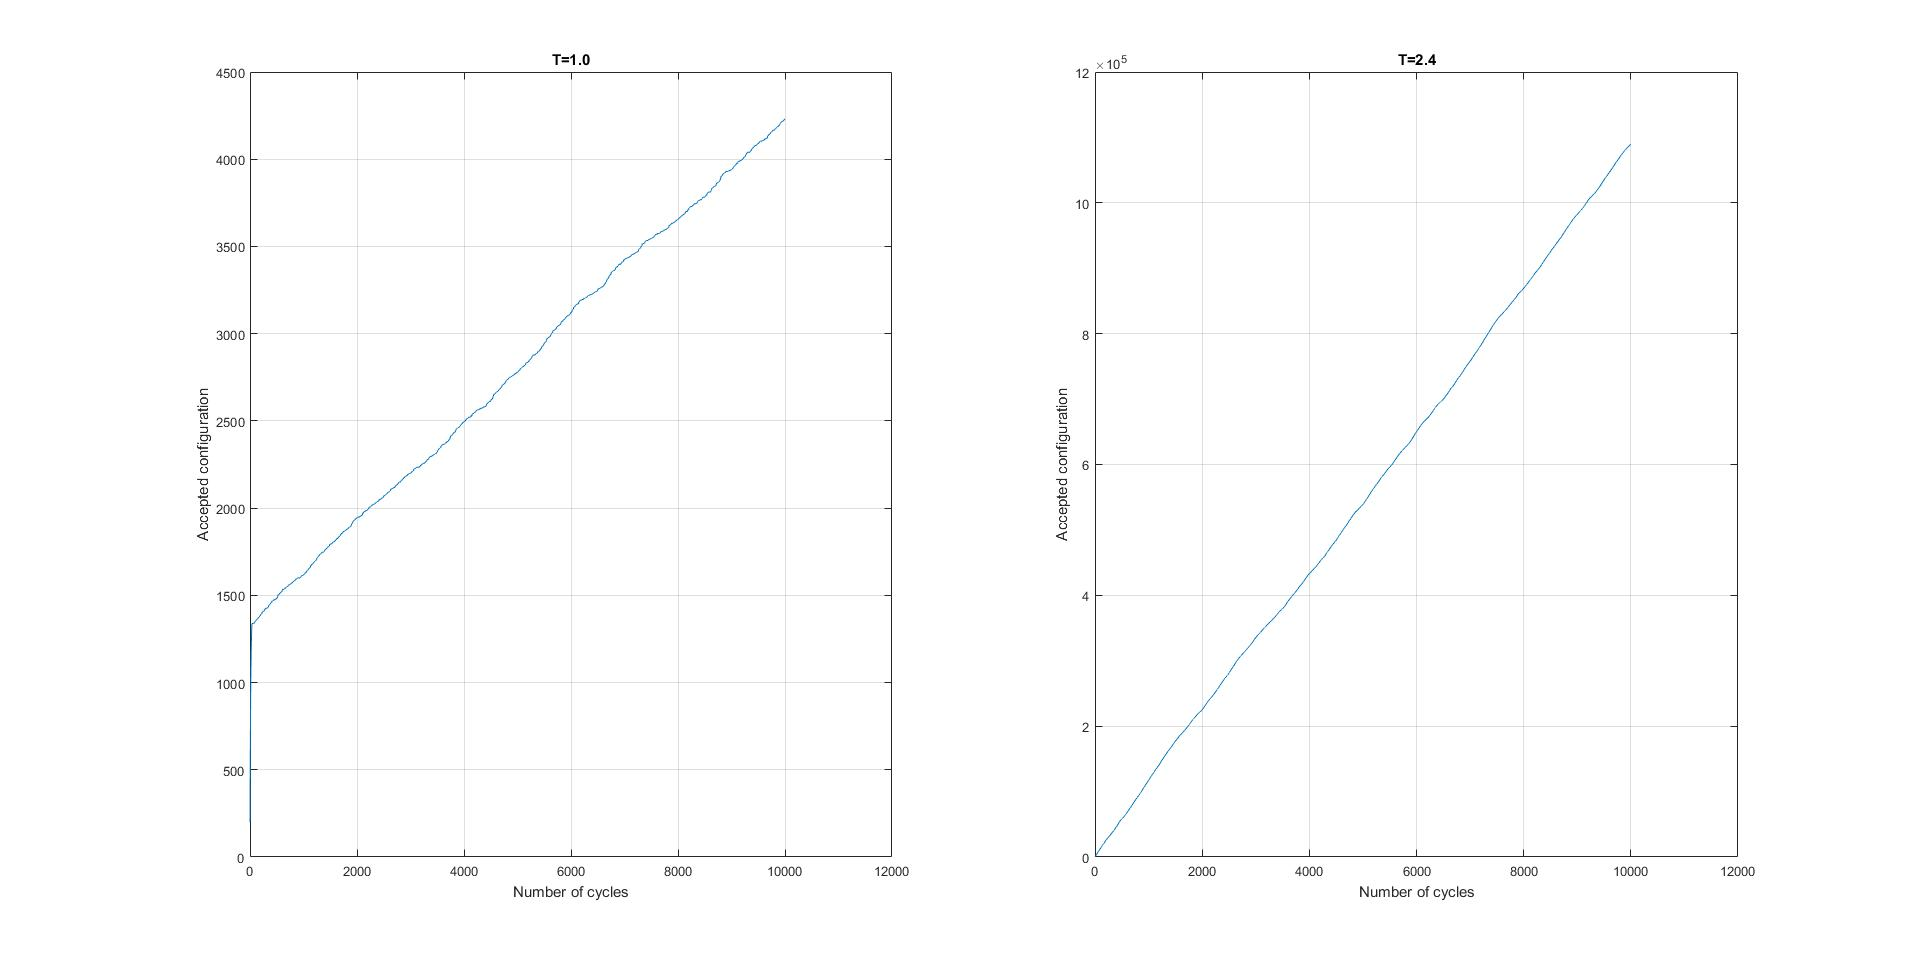
\includegraphics[scale=0.245]{randomaccept.jpg}
}
\caption{Number of accepted configurations for a random initial matrix computed with $10^4$ Monte Carlo cycles for $T=1.0$ and $T=2.4$.}
\label{fig:RandomAccept}
\end{figure}

\begin{figure} [H]
\centerline{
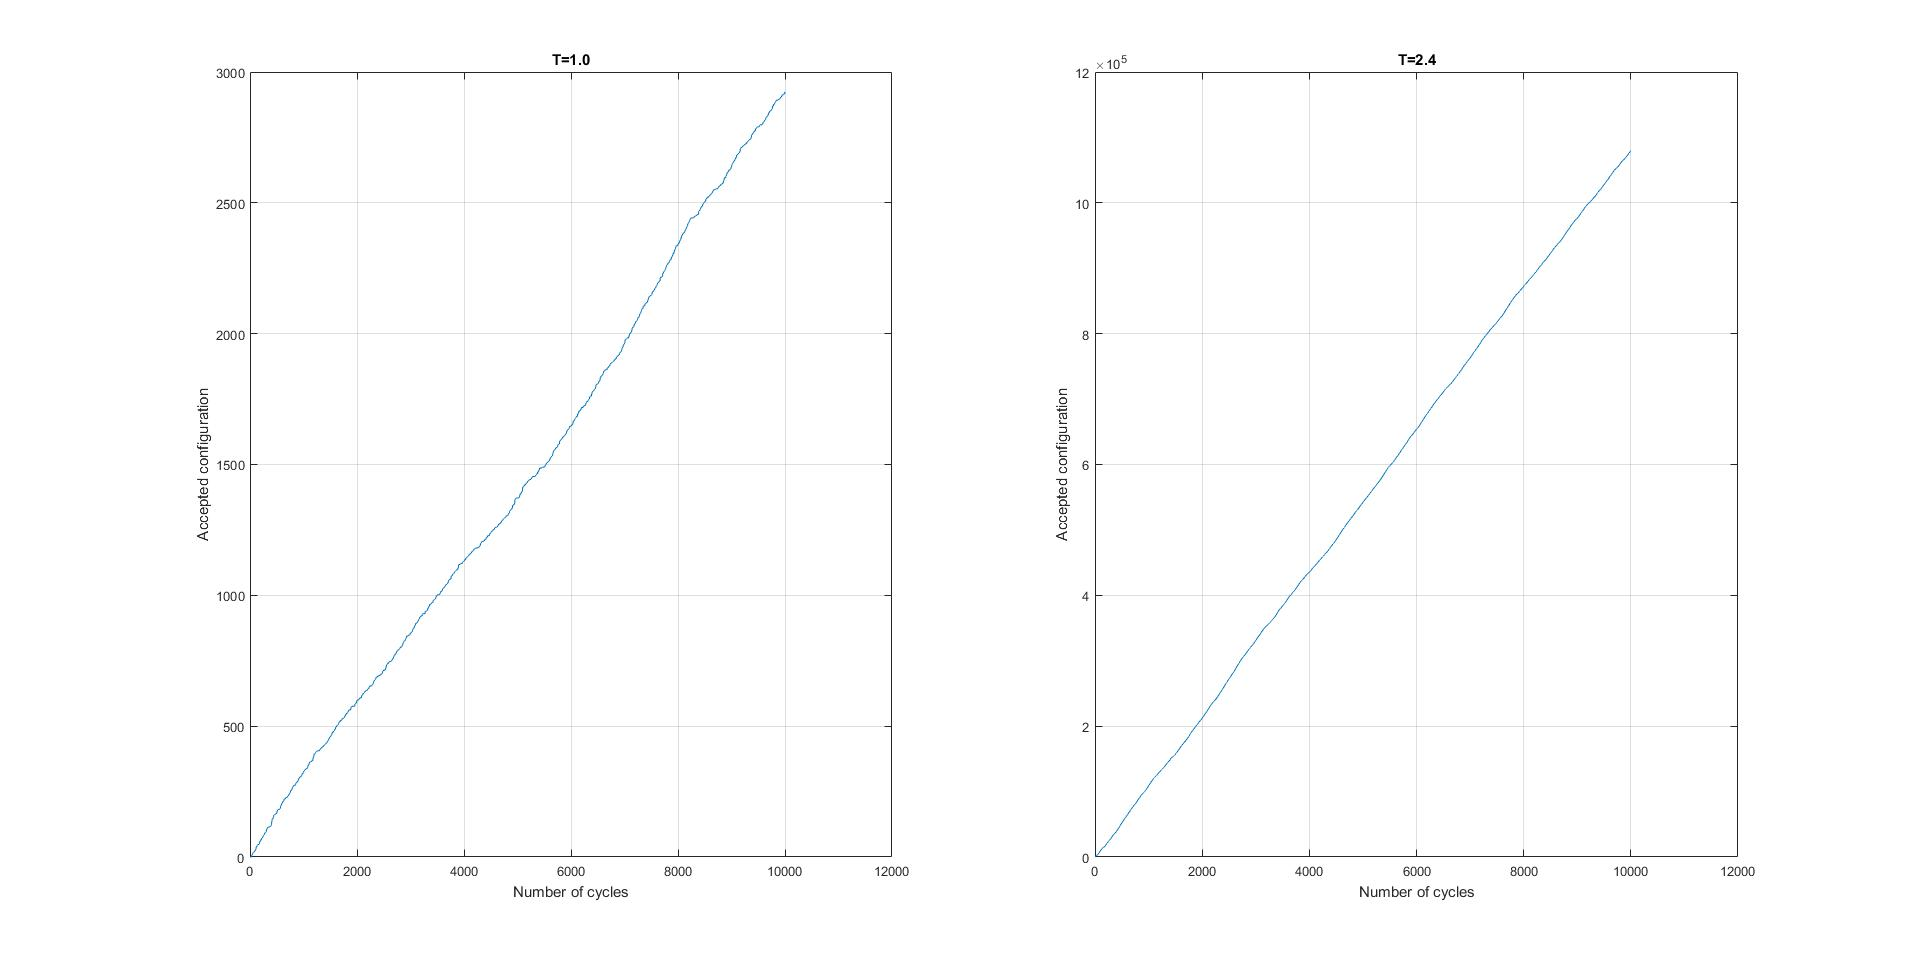
\includegraphics[scale=0.245]{upaccept.jpg}
}
\caption{Number of accepted configurations for an all up initial matrix computed with $10^4$ Monte Carlo cycles for $T=1.0$ and $T=2.4$.}
\label{fig:UpAccept}
\end{figure}
\noindent The system with a random initial matrix at $T=1.0$ accepts many flips in the first few Monte Carlo cycles (\figref{RandomAccept}). This is because it initially is not at the equilibrium state. After it has reached equilibrium, it accepts far fewer moves, and follows the same pattern as \figref{UpAccept} A. When subtracting the number of accepted configurations from the first few cycles in \figref{RandomAccept} A from the total number of accepted configurations, the answer is the same number of accepted configurations as in \figref{UpAccept} A. The total number of accepted configurations is much higher when $T=2.4$, and the difference is negligible between the two.

\newpage 
\begin{figure}
\centerline{
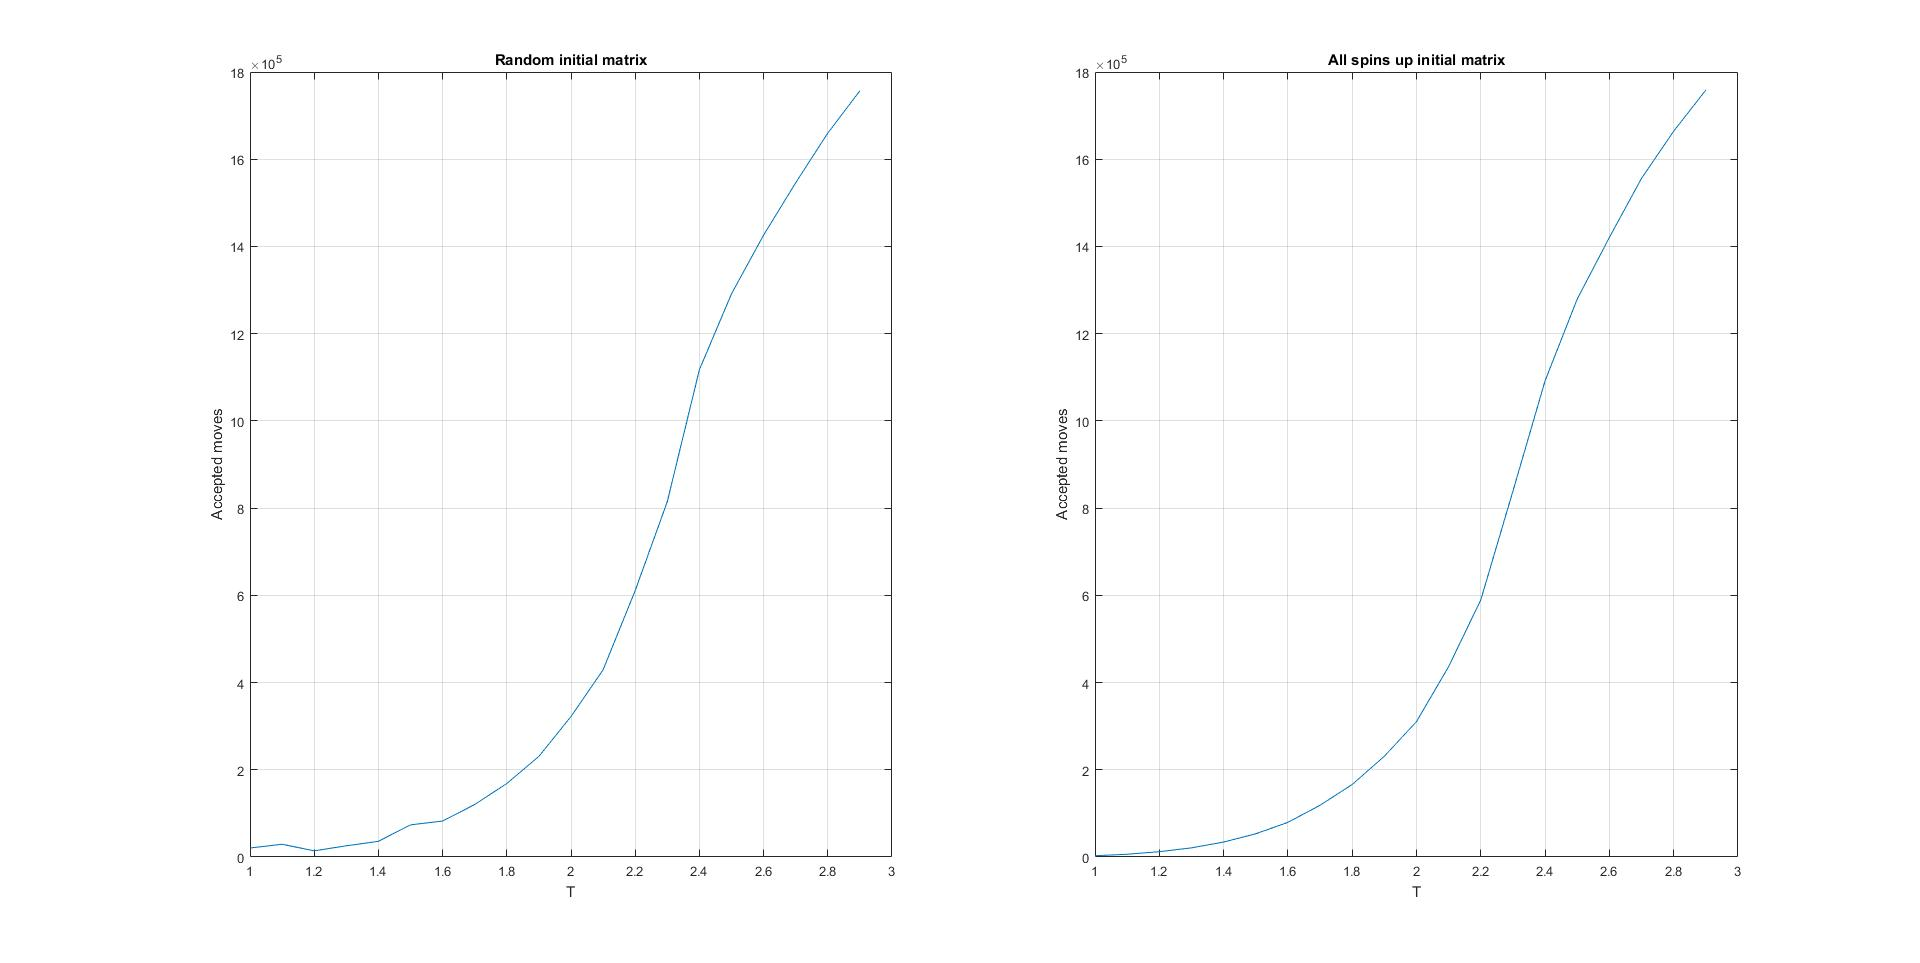
\includegraphics[scale=0.275]{accept.jpg}
}
\caption{Total number of accepted configurations as a function of temperature}
\label{fig:Accept}
\end{figure}
\noindent The number of configurations grows exponentially with temperature. The smooth nature of the all spins up initial matrix is contrasted by the graph for a random initial matrix. The uneven nature of this graph is a result of the random initial matrix. 


\begin{figure}
\centerline{
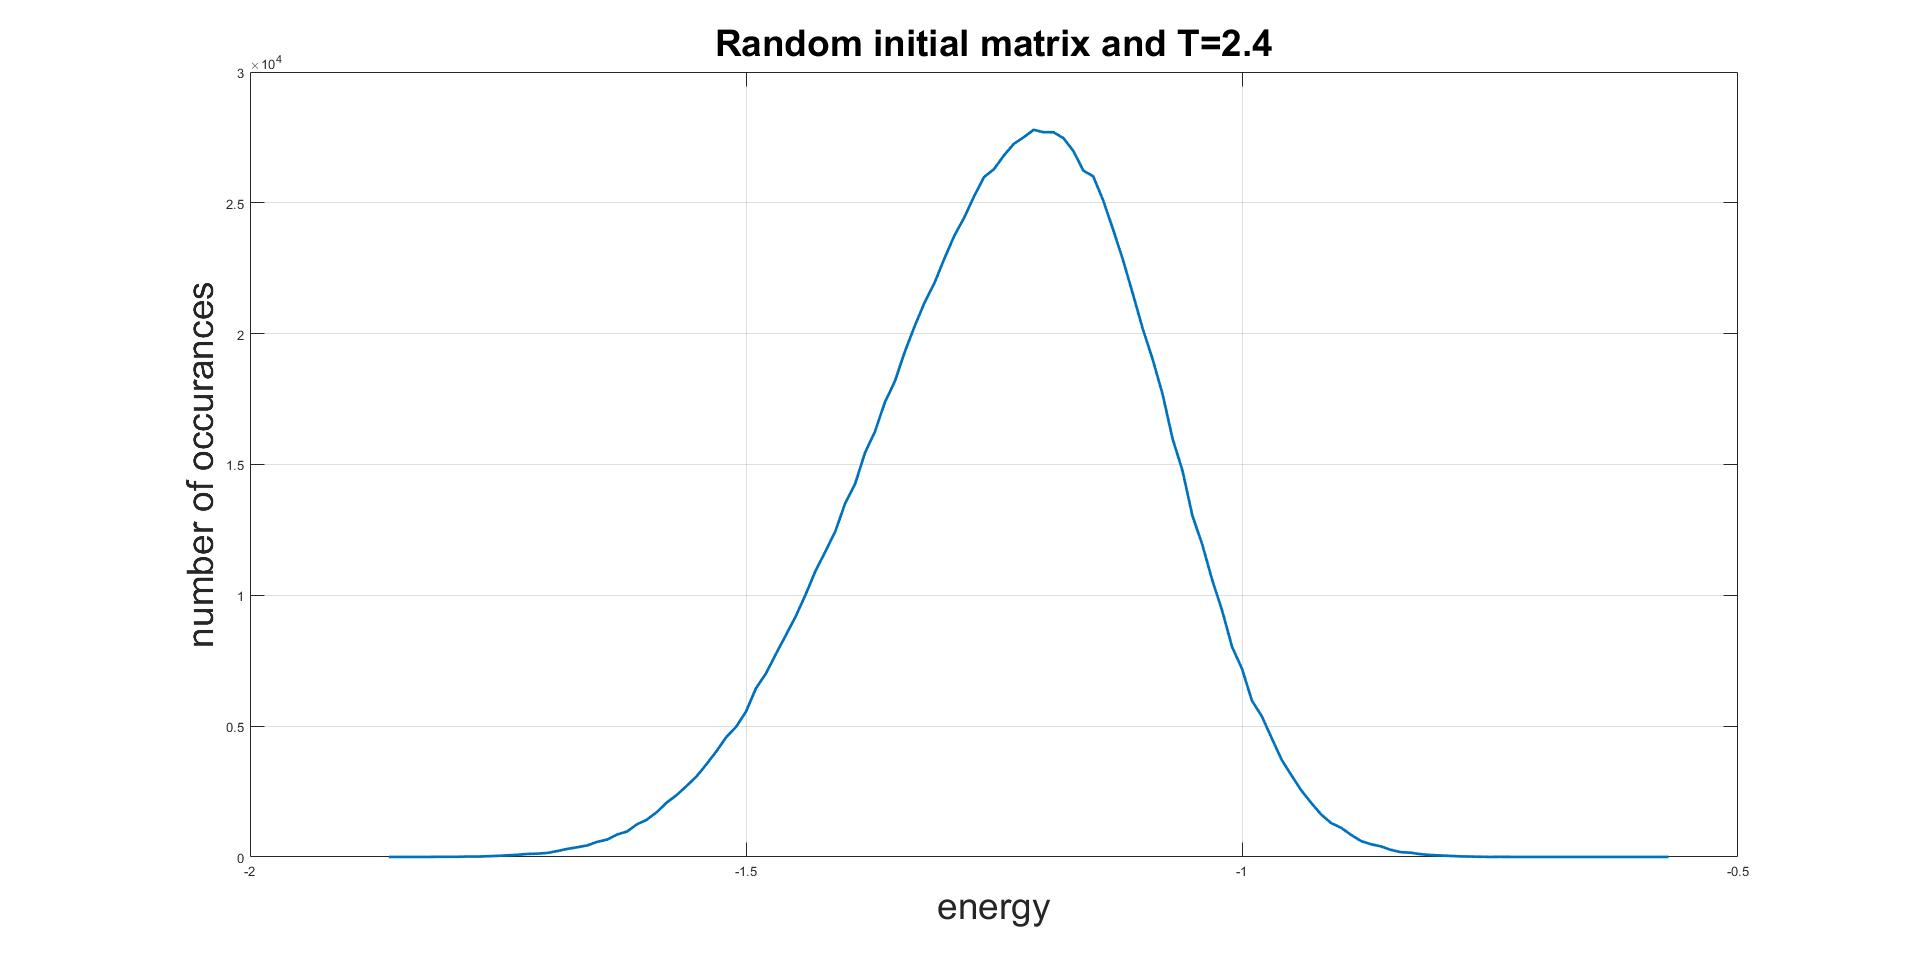
\includegraphics[scale=0.15]{OccurancesRandom.jpg}
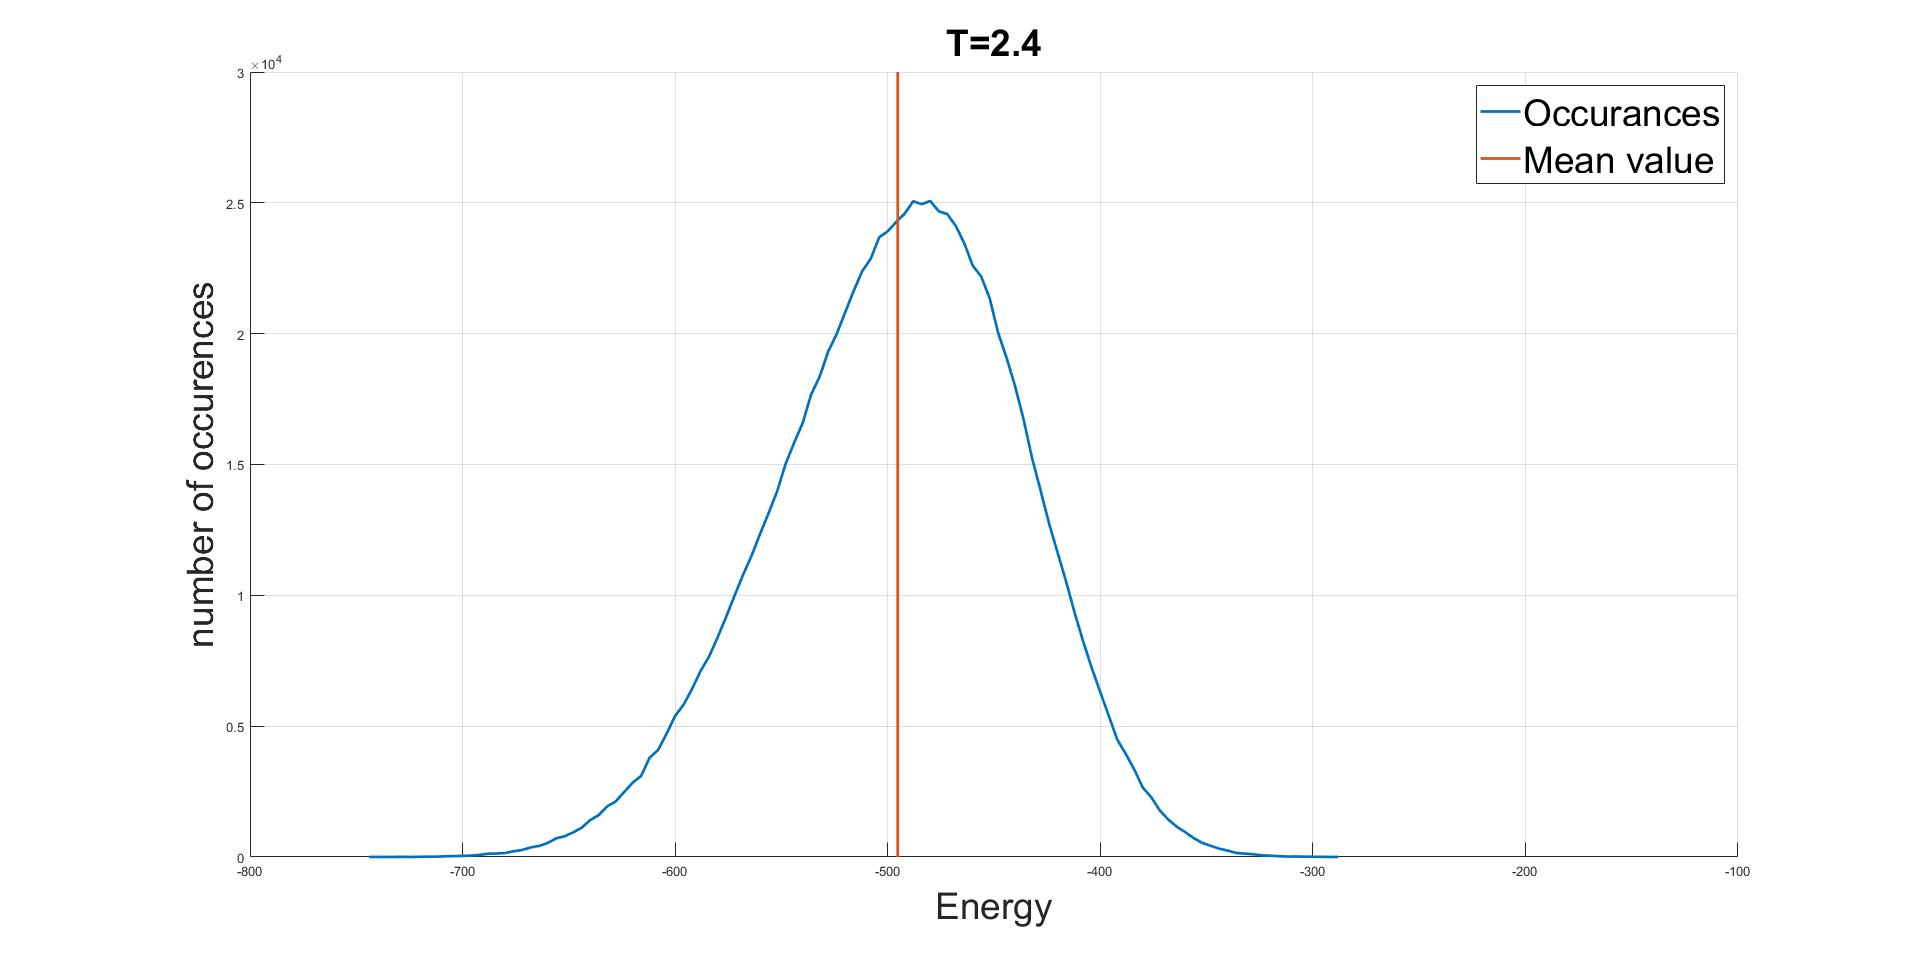
\includegraphics[scale=0.15]{OccurancesUp.jpg}
}
\caption{Probability distribution for T=2.4 for a random and an all up initial matrix.}
\label{fig:ProbBoth}
\end{figure}

\begin{figure} [H]
\centerline{
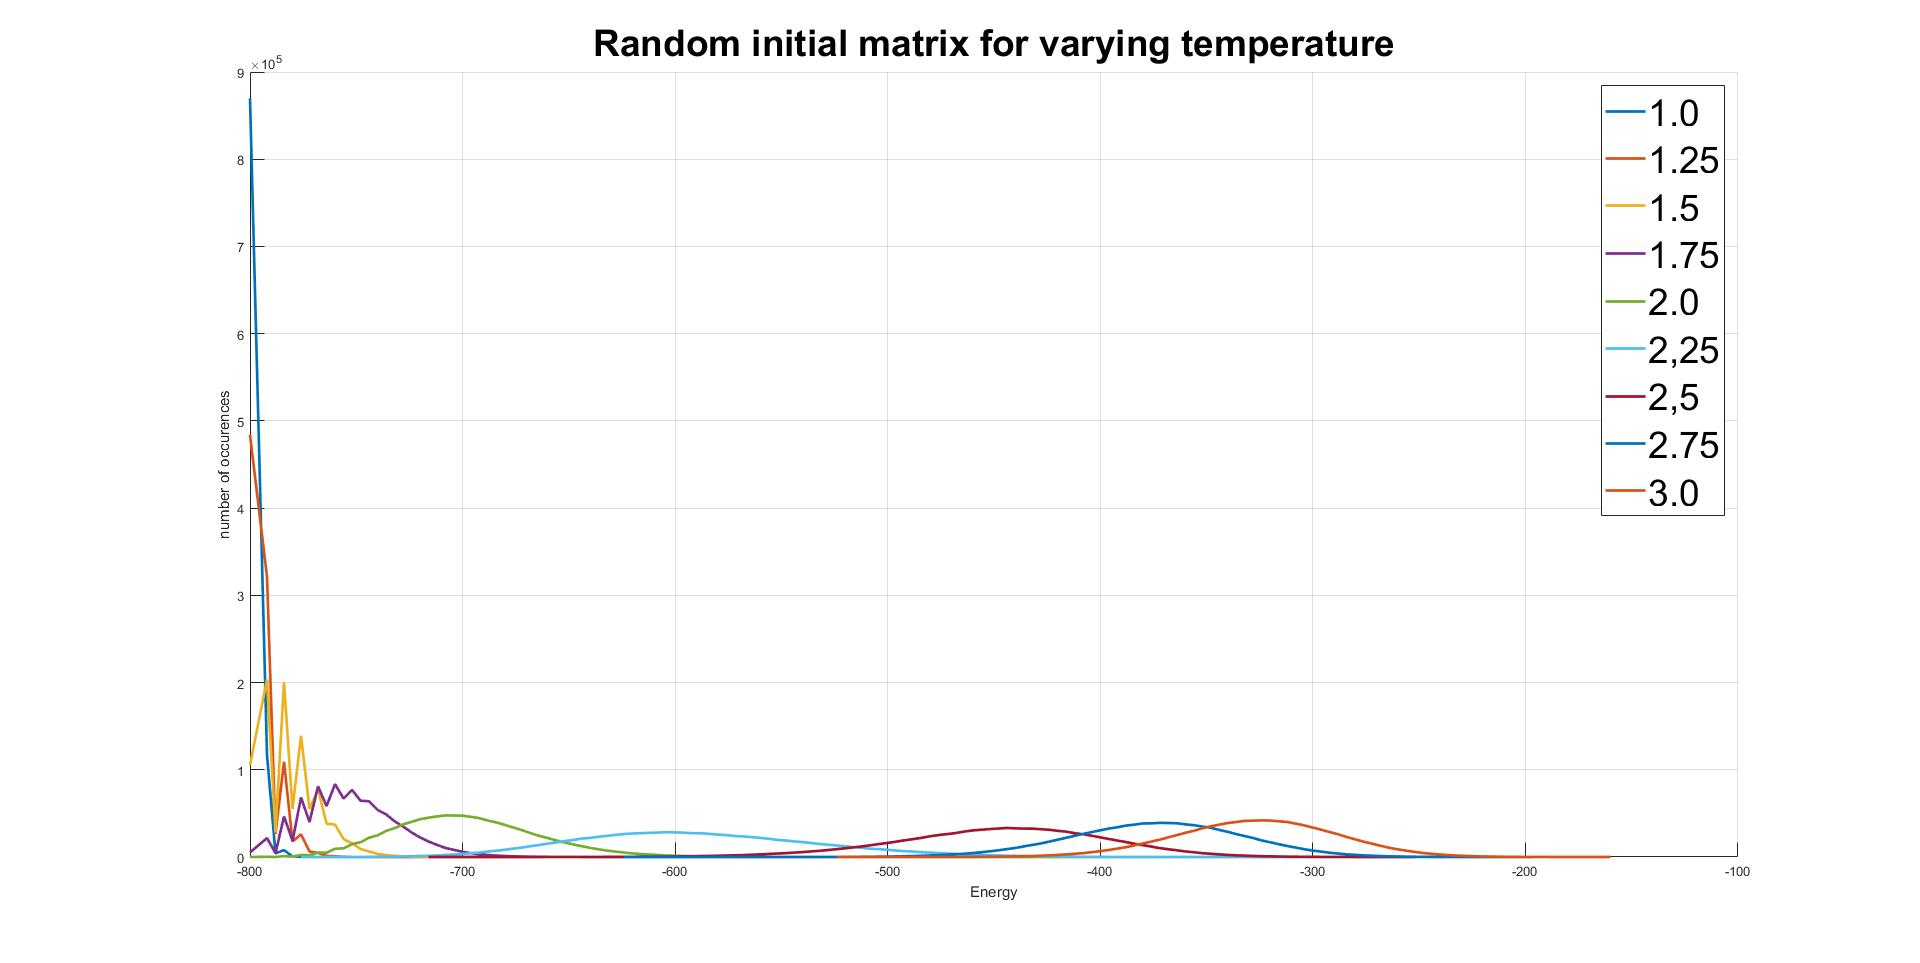
\includegraphics[scale=0.30]{ProbabilityRandom.jpg}
}
\caption{Probability distribution for varying temperature. Computed with $10^6$ Monte Carlo cycles.}
\label{fig:Probability}
\end{figure}

\begin{center}
\textbf{Table 3:} Variance in energy for different temperatures computed with a random matrix for different temperatures and $10^6$ Monte carlo cycles.
\end{center}
\centerline{
\begin{tabular}{|l|c|}
\hline
  Temperature & Variance\\
\hline
  T=1.0 & 10.1076\\
\hline
  T=1.25 & 52.9558\\
\hline
  T=1.50 & 181.261\\
\hline
  T=1.75 & 478.219\\
\hline
  T=2.0 & 1157.08\\
\hline 
  T=2.25 & 3145.36\\
\hline 
  T= 2.50 & 2479.22 \\
\hline 
  T=2.75 & 1690.69\\
\hline
  T=3.0 & 1445.91\\
\hline
\end{tabular}
}

\noindent The probability distribution shown in \figref{Probability} show that higher energies are to be expected when the temperature is increased. When the temperature is low, there are only a few possible energy states. This is in accordance with the energyplots in \figref{RandomEnergy} and \figref{UpEnergy}. The variance in table 3 is increasing up to $T=2.25$ before decreasing again. This is also shown in \figref{Probability}. The graph representing $T=2.25$ is much wider than all the other graphs. The probability distribution for $T=2.4$ is shown in \figref{ProbBoth}. The graph is skewed towards higher energies. WHY ARE THEY SKEWED?

For T mindre og lik 2.25 er de skewed positivt, og negativt for t større enn 2.25

  





\newpage
{\LARGE\bf
Discussion 
}

For the $2 \times 2$ case, the expection values showed distinct sensitivities (table 1,2). The mean energy and mean absolute magnetization converged quickly towards the analytic value. Both were accurate with three leading digits for as few as $10^4$ Monte Carlo cycles. When increasing the number of Monte Carlo cycles to $10^6$ the relative error decreases to a fraction of a $\permil$. The specific heat and susceptibility were both sensitive. The specific heat was accurate up to two or three leading digits, depending on the starting matrix, when computed with $10^6$ Monte Carlo cycles. The specific heat was accurate up to only one or two leading digits with $10^6$ Monte Carlo cycles. The program did not produce the same results for each run. This is due to the random nature of the system being examined.

The $20 \times 20$ case was studied with an emphasis on the energy and magnetization for $T=1.0$ and $T=2.4$
  








\newpage
{\LARGE\bf
Conclusion
}
















\newpage
{\LARGE\bf
Reference list
}\\
Hjort-Jensen,M., 2015. Computational physics, accessible at course github repository. 551 pages

\end{document}